% Options for packages loaded elsewhere
\PassOptionsToPackage{unicode}{hyperref}
\PassOptionsToPackage{hyphens}{url}
%
\documentclass[
]{article}
\usepackage{amsmath,amssymb}
\usepackage{lmodern}
\usepackage{iftex}
\ifPDFTeX
  \usepackage[T1]{fontenc}
  \usepackage[utf8]{inputenc}
  \usepackage{textcomp} % provide euro and other symbols
\else % if luatex or xetex
  \usepackage{unicode-math}
  \defaultfontfeatures{Scale=MatchLowercase}
  \defaultfontfeatures[\rmfamily]{Ligatures=TeX,Scale=1}
\fi
% Use upquote if available, for straight quotes in verbatim environments
\IfFileExists{upquote.sty}{\usepackage{upquote}}{}
\IfFileExists{microtype.sty}{% use microtype if available
  \usepackage[]{microtype}
  \UseMicrotypeSet[protrusion]{basicmath} % disable protrusion for tt fonts
}{}
\makeatletter
\@ifundefined{KOMAClassName}{% if non-KOMA class
  \IfFileExists{parskip.sty}{%
    \usepackage{parskip}
  }{% else
    \setlength{\parindent}{0pt}
    \setlength{\parskip}{6pt plus 2pt minus 1pt}}
}{% if KOMA class
  \KOMAoptions{parskip=half}}
\makeatother
\usepackage{xcolor}
\usepackage[margin=1in]{geometry}
\usepackage{color}
\usepackage{fancyvrb}
\newcommand{\VerbBar}{|}
\newcommand{\VERB}{\Verb[commandchars=\\\{\}]}
\DefineVerbatimEnvironment{Highlighting}{Verbatim}{commandchars=\\\{\}}
% Add ',fontsize=\small' for more characters per line
\usepackage{framed}
\definecolor{shadecolor}{RGB}{248,248,248}
\newenvironment{Shaded}{\begin{snugshade}}{\end{snugshade}}
\newcommand{\AlertTok}[1]{\textcolor[rgb]{0.94,0.16,0.16}{#1}}
\newcommand{\AnnotationTok}[1]{\textcolor[rgb]{0.56,0.35,0.01}{\textbf{\textit{#1}}}}
\newcommand{\AttributeTok}[1]{\textcolor[rgb]{0.77,0.63,0.00}{#1}}
\newcommand{\BaseNTok}[1]{\textcolor[rgb]{0.00,0.00,0.81}{#1}}
\newcommand{\BuiltInTok}[1]{#1}
\newcommand{\CharTok}[1]{\textcolor[rgb]{0.31,0.60,0.02}{#1}}
\newcommand{\CommentTok}[1]{\textcolor[rgb]{0.56,0.35,0.01}{\textit{#1}}}
\newcommand{\CommentVarTok}[1]{\textcolor[rgb]{0.56,0.35,0.01}{\textbf{\textit{#1}}}}
\newcommand{\ConstantTok}[1]{\textcolor[rgb]{0.00,0.00,0.00}{#1}}
\newcommand{\ControlFlowTok}[1]{\textcolor[rgb]{0.13,0.29,0.53}{\textbf{#1}}}
\newcommand{\DataTypeTok}[1]{\textcolor[rgb]{0.13,0.29,0.53}{#1}}
\newcommand{\DecValTok}[1]{\textcolor[rgb]{0.00,0.00,0.81}{#1}}
\newcommand{\DocumentationTok}[1]{\textcolor[rgb]{0.56,0.35,0.01}{\textbf{\textit{#1}}}}
\newcommand{\ErrorTok}[1]{\textcolor[rgb]{0.64,0.00,0.00}{\textbf{#1}}}
\newcommand{\ExtensionTok}[1]{#1}
\newcommand{\FloatTok}[1]{\textcolor[rgb]{0.00,0.00,0.81}{#1}}
\newcommand{\FunctionTok}[1]{\textcolor[rgb]{0.00,0.00,0.00}{#1}}
\newcommand{\ImportTok}[1]{#1}
\newcommand{\InformationTok}[1]{\textcolor[rgb]{0.56,0.35,0.01}{\textbf{\textit{#1}}}}
\newcommand{\KeywordTok}[1]{\textcolor[rgb]{0.13,0.29,0.53}{\textbf{#1}}}
\newcommand{\NormalTok}[1]{#1}
\newcommand{\OperatorTok}[1]{\textcolor[rgb]{0.81,0.36,0.00}{\textbf{#1}}}
\newcommand{\OtherTok}[1]{\textcolor[rgb]{0.56,0.35,0.01}{#1}}
\newcommand{\PreprocessorTok}[1]{\textcolor[rgb]{0.56,0.35,0.01}{\textit{#1}}}
\newcommand{\RegionMarkerTok}[1]{#1}
\newcommand{\SpecialCharTok}[1]{\textcolor[rgb]{0.00,0.00,0.00}{#1}}
\newcommand{\SpecialStringTok}[1]{\textcolor[rgb]{0.31,0.60,0.02}{#1}}
\newcommand{\StringTok}[1]{\textcolor[rgb]{0.31,0.60,0.02}{#1}}
\newcommand{\VariableTok}[1]{\textcolor[rgb]{0.00,0.00,0.00}{#1}}
\newcommand{\VerbatimStringTok}[1]{\textcolor[rgb]{0.31,0.60,0.02}{#1}}
\newcommand{\WarningTok}[1]{\textcolor[rgb]{0.56,0.35,0.01}{\textbf{\textit{#1}}}}
\usepackage{graphicx}
\makeatletter
\def\maxwidth{\ifdim\Gin@nat@width>\linewidth\linewidth\else\Gin@nat@width\fi}
\def\maxheight{\ifdim\Gin@nat@height>\textheight\textheight\else\Gin@nat@height\fi}
\makeatother
% Scale images if necessary, so that they will not overflow the page
% margins by default, and it is still possible to overwrite the defaults
% using explicit options in \includegraphics[width, height, ...]{}
\setkeys{Gin}{width=\maxwidth,height=\maxheight,keepaspectratio}
% Set default figure placement to htbp
\makeatletter
\def\fps@figure{htbp}
\makeatother
\setlength{\emergencystretch}{3em} % prevent overfull lines
\providecommand{\tightlist}{%
  \setlength{\itemsep}{0pt}\setlength{\parskip}{0pt}}
\setcounter{secnumdepth}{-\maxdimen} % remove section numbering
\ifLuaTeX
  \usepackage{selnolig}  % disable illegal ligatures
\fi
\IfFileExists{bookmark.sty}{\usepackage{bookmark}}{\usepackage{hyperref}}
\IfFileExists{xurl.sty}{\usepackage{xurl}}{} % add URL line breaks if available
\urlstyle{same} % disable monospaced font for URLs
\hypersetup{
  pdftitle={FinalReport},
  hidelinks,
  pdfcreator={LaTeX via pandoc}}

\title{FinalReport}
\author{}
\date{\vspace{-2.5em}}

\begin{document}
\maketitle

\hypertarget{i.-introduction}{%
\section{I. INTRODUCTION}\label{i.-introduction}}

\textbf{1.1} The European Social Survey According to the official
website of the European Social Survey (ESS), the ESS is a survey
conducted academically across Europe every two-year on a cross-national
basis since 2001 through face-to-face interviews. Variables measured in
this survey include the attitudes, beliefs and behaviour patterns of
diverse populations. Its three main aims are, to monitor and interpret
changing public attitudes and values within Europe and to investigate
how they interact with Europe's changing institutions, to advance and
consolidate improved methods of cross-national survey measurement in
Europe and beyond, and to develop a series of European social
indicators, including attitudinal indicators.

Until now, the ESS has had ten rounds, the first round conducted in 2002
and the tenth round in 2020. For analysis in this report, we will use
data from the ninth round. In the ninth round, the survey covers 30
countries and employs the most rigorous methodologies funded by the
Members, Observers and Guests of the ESS European Research
Infrastructure Consortium (ESS ERIC) who represent national governments.

The survey involves strict random probability sampling with a minimum
target response rate of 70\% and rigorous translation protocols. The
hour-long face-to-face interview includes questions on a variety of core
topics repeated from previous rounds of the survey and also two modules
developed for Round 9 covering Justice and Fairness in Europe, and the
Timing of Life (the latter is a partial repeat of a module from Round
3).

The scope of this survey is all persons aged 15 and over resident within
private households, regardless of their nationality, citizenship,
language or legal status, in the listed countries conducted from August
30, 2018, to January 27, 2020. The listed countries in the ninth round
are Albania, Austria, Belgium, Bulgaria, Croatia, Cyprus, Czechia,
Denmark, Estonia, Finland, France, Germany, Germany, Hungary, Iceland,
Ireland, Italy, Latvia, Lithuania, Montenegro, Netherlands, Norway,
Poland, Portugal, Romania, Serbia, Slovakia, Slovenia, Spain, Sweden,
Sweden, Switzerland, United Kingdom.

By exploring the documentation file, we found that in the ninth round,
there are four weights in this survey. Design Weights The purpose of the
design weights (DWEIGHT) is to correct for unequal probabilities for
selection due to the sampling design used. In general design weights
were computed for each country as follows. w =
1/(PROB1\emph{\ldots{}}PROBk) is a nx1 vector of weights; k depends on
the number of stages of the sampling design. All weights were rescaled
in a way that the sum of the final weights equals n, i.e.~rescaled
weights = n\emph{w/sum(w). It is not recommended to use this weight
without non-response correction. Post-stratification Weights The purpose
of the post-stratified design weights (PSPWGHT) is to reduce sampling
error, non-coverage, and non-response bias, using auxiliary information
specified by the sampling design. The post-stratification targets use
information about age, gender, education and region. Raking (iterative
proportional fitting) has been used in the production of the
post-stratified weights. It also takes into account differences in
population size across countries. Analysis Weights The analysis weight
(ANWEIGHT) corrects for population size when combining two or more
countries' data, and is calculated as ANWEIGHT=PSPWGHT}PWEIGHT. This is
a weight in all analyses, it is constructed by first deriving the design
weight, then applying a post-stratification adjustment, and then a
population size adjustment. Population Weights The Population size
weight (PWEIGHT) corrects for population size when combining two or more
country's data, and is calculated as PWEIGHT={[}Population aged 15 years
and over{]}/{[}(Net sample in data file)*10 000{]}

\textbf{1.2} Objective The purpose of this report is to impute missing
values in the variable HINCTNTA. This variable is household income in
deciles. The categories in variable HINCTNTA are national and based on
deciles of the actual household income range in the given country. These
deciles are derived from different sources. The median income is the
reference point and the 10 deciles are calculated with the median itself
at the top of the fifth decile (category F).

\hypertarget{ii.-missing-data-challenge}{%
\section{II. MISSING DATA CHALLENGE}\label{ii.-missing-data-challenge}}

\textbf{2.1} Select five countries Here, we limit to five countries only
to impute missing values. The five countries are selected randomly. The
selected countries are Austria, Ireland, Portugal, Hungary, and Poland.
These countries have different sources. In Austria and Portugal, it
refers to annual household income with a lower limit is €15,300 €5,636
and an upper limit is €77,500 and €35,092, respectively. In Ireland, it
refers to weekly household income with an upper limit of €1,680 and a
lower limit of €270. Differently, in Hungary and Poland, household
income refers to monthly income with a lower limit and an upper limit in
Hungary Ft130,000 and Ft410,000 and zł1,700 and zł8,801 in Poland,
respectively.

The missing values themselves have three different types, which are
refusal, don't know, and no answer and coded differently. Here are the
bar charts of five countries to show the frequency of missing values and
each decile group.

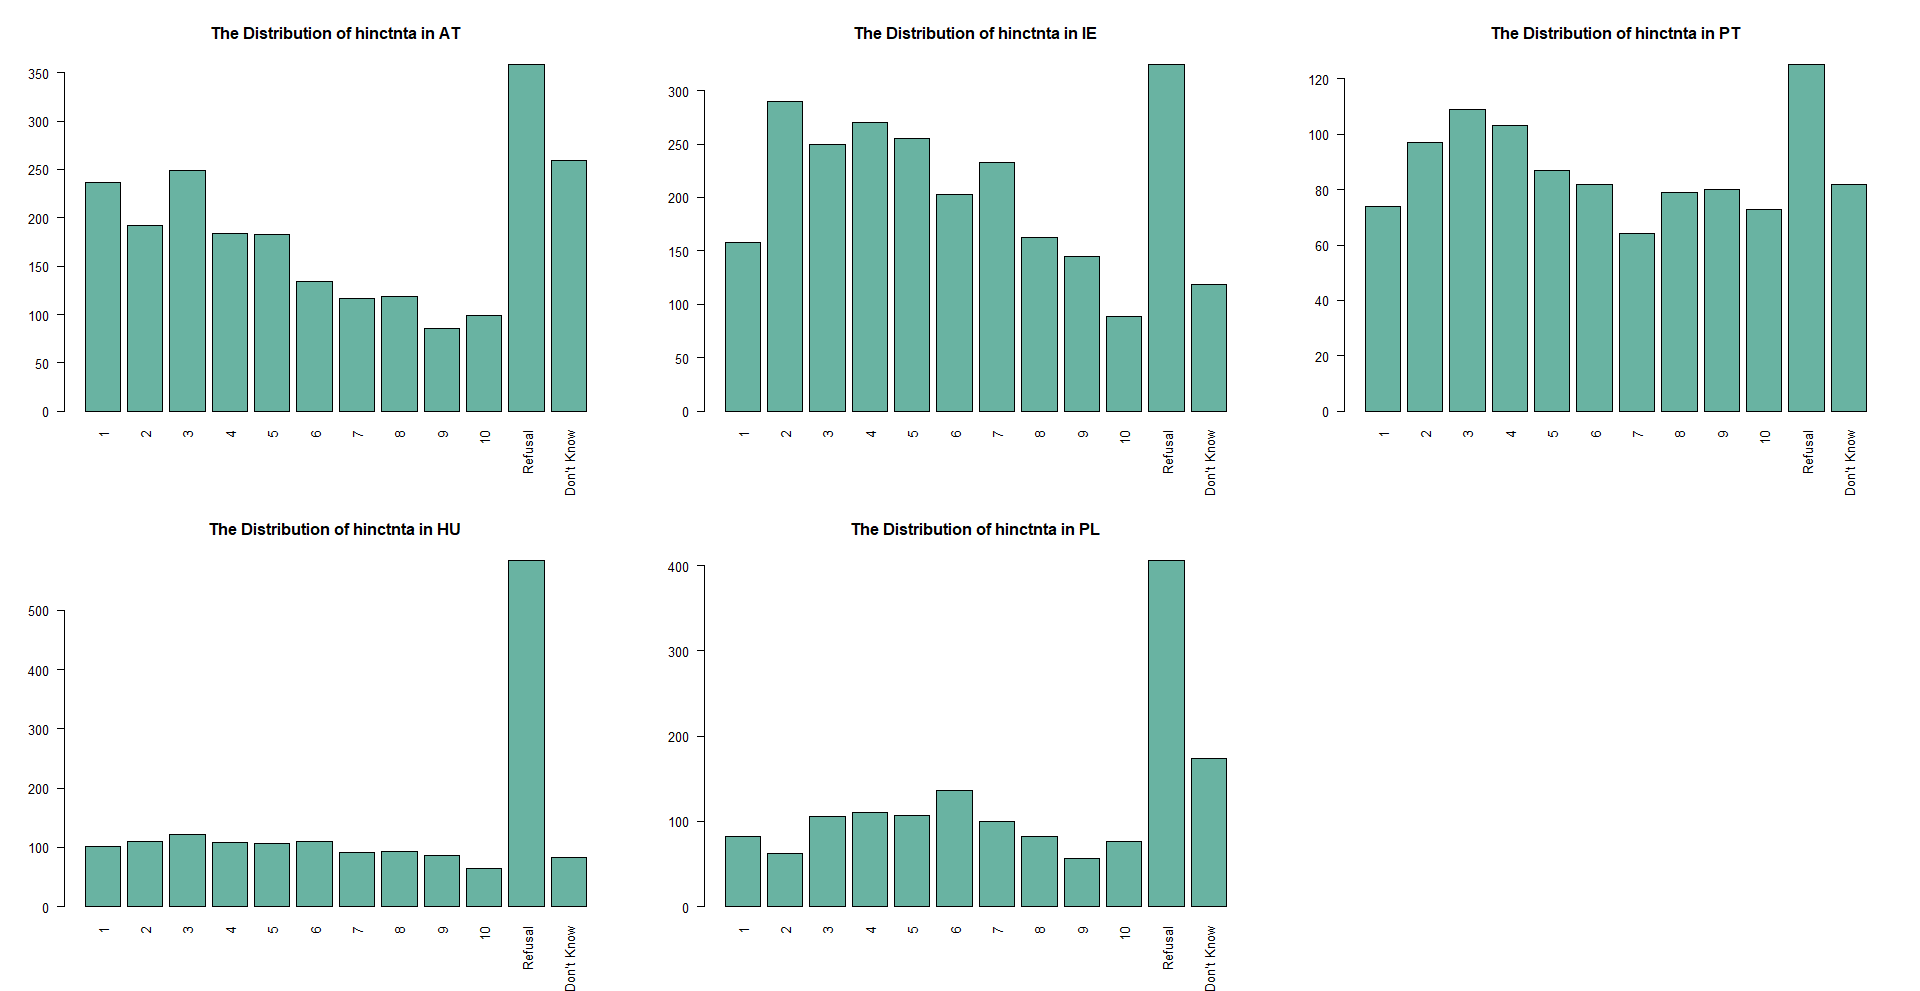
\includegraphics[width=1\linewidth]{pics/plot_zoom}

\textbf{2.2} Missing values imputation In order to fix missing values
across countries, we decided to impute every country separately for some
reasons. First, the variable HINCTNTA itself is differently distributed
for every country, so simultaneous imputation would not make sense. This
is also in line with other studies (Plumpton et al., 2016; Sintonen et
al., 2016; Dorsch \& Maarek, 2019; Weber \& Denk, 2011; Landrum \&
Becker, 2001). Another thing is, not only is HINCTNTA differently
distributed but the variable is divided into deciles, as can be seen in
the plots, meaning that the range also differs for every country.

As we know, the income variable is a continuous variable. However, what
we have here is in an ordinal scale because it is grouped as deciles.
Since the incomes are reported as deciles rather than the raw values,
where each decile contains 10\% of incomes in a country, this may yield
some difficulties when imputing the variable. One option would be to
treat the variables as nominal and then use polynomial regression to
impute the income classes, but this would ignore the ordering of the
variable and thus come with more difficulties.

Ryder et al.~(2011) recommend using the midpoint for each income class
as a surrogate to be used for imputation so that the variable can be
treated as a continuous variable. For instance, in an income class
indicating €10000 - €16000, €13000 will be used as a surrogate.

If we then use predictive mean matching as an imputation method, only
observed values are used as possible imputed values, and thus these
imputed values can again be transformed to the established income
classes after imputation. Predictive mean matching is a hot deck method
that calculates the predicted value of the target variable based on the
specified imputation model. The method establishes a small set of
potential donors for each missing data from all complete cases that has
the closest predicted value to the predicted value for the missing data
then a random donor is taken from the candidate to replace the missing
value assuming the missing data and observed data have the same
distribution (van Buuren, 2018).

In the previous section, we also mentioned that there are weights
included as variables in this survey. Based on previous research,
weights are included to fix missing values. Quartagno et al.~(2020) used
an imputation model where the weights are included as additional
variables. Kim et al.~(2006) and Seaman et al.~(2012) suggested a better
imputation model should include not only the weights but also all
interactions between weights and covariates. This can be done easily
when missing data are confined to the outcome variable---but not when
data are missing in all variables. Andridge and Little (2009) used the
sampling weight as a stratifying variable alongside additional
adjustment variables when forming adjustment cells (hot deck
imputations).

From the four kinds of weights, we only use analysis weight (ANWEIGHT)
as a predictor variable because this is a weight in all analyses and can
correct population size when combining more than one country. In
addition to the analysis weight, we will use ten variables and
interactions between those variables with the weight. The variables used
are chosen based on the previous studies and rational reasoning.

\begin{enumerate}
\def\labelenumi{\arabic{enumi}.}
\tightlist
\item
  PDWRK: partner doing paid work last 7 days

  \begin{itemize}
  \tightlist
  \item
    Household income meaning income from for all workers in a household.
    We assume that if respondent's partner is an active worker within
    the last 7 days then it will influence the total household income.
  \end{itemize}
\item
  BTHCLD: ever given birth to/ fathered a child

  \begin{itemize}
  \tightlist
  \item
    According to Kolk (2021), fertility for both men and women groups
    have positive relationship. It mentioned that men and women with two
    or more children have higher income than people with one or no
    child.
  \end{itemize}
\item
  GNDR: gender of respondents

  \begin{itemize}
  \tightlist
  \item
    Based on data from International Monetary Fund (2015), more men work
    than women in most countries and they get paid more for similar
    work. Therefore, respondent's gender obviously has relationship with
    the household income.
  \end{itemize}
\item
  MARITALB: legal marital status

  \begin{itemize}
  \tightlist
  \item
    Ideally, legal marital status has relationship with the household
    income. It is inline with study from Balcazar (2019) that mentioned
    married individuals have the highest incomes level out of all groups
    (single, married, divorce, separated, never married). Moreover,
    unmarried couple in some countries counted as separate households.
  \end{itemize}
\item
  LRSCALE: placement on left right scale

  \begin{itemize}
  \tightlist
  \item
    We take self-placement of Left-Right into consideration because
    household income is a significant predictor of respondent's
    Left-Right self-placement, controlling all other variables (Esposito
    \& Theuerkauf, 2021). It also mentioned a positive sign of income
    indicates that one's perception of family prosperity is related to
    one's placement on the right side of the ceteris paribus scale.
  \end{itemize}
\item
  DSCRGRP: member of a group discriminated against in this country
\item
  HHMMB: number of people living regularly as member of household
\item
  AGEA: age of respondents
\item
  WKHTOT: total hours normally worked per week in main job overtime
  included
\item
  EISCED: highest level of education
\end{enumerate}

(PDWRK), (BTHCLD), (GNDR), (MARITALB), (LRSCALE), (DSCRGRP), (HHMMB),
(AGEA), (WKHTOT), (EISCED).

\hypertarget{iii.-methodology-and-results}{%
\section{III. Methodology and
Results}\label{iii.-methodology-and-results}}

\hypertarget{input-data-and-packages}{%
\subsection{3.1 Input data and packages}\label{input-data-and-packages}}

\begin{Shaded}
\begin{Highlighting}[]
\CommentTok{\#devtools::install\_github("amices/ggmice")}
\FunctionTok{library}\NormalTok{(tidyverse)}
\FunctionTok{library}\NormalTok{(mice)}
\FunctionTok{library}\NormalTok{(ggmice)}
\FunctionTok{library}\NormalTok{(psych)}
\FunctionTok{library}\NormalTok{(visdat)}

\CommentTok{\#Input Data}
\NormalTok{ess }\OtherTok{\textless{}{-}} \FunctionTok{readRDS}\NormalTok{(}\StringTok{"Ess round 9.RDS"}\NormalTok{)}
\end{Highlighting}
\end{Shaded}

\hypertarget{data-processing}{%
\subsection{3.2 Data processing}\label{data-processing}}

In order to obtain the data of the 5 chosen countries, we have to divide
the original data.

\begin{Shaded}
\begin{Highlighting}[]
\CommentTok{\#Find the column full of NAs}
\NormalTok{findNACol }\OtherTok{\textless{}{-}} \ControlFlowTok{function}\NormalTok{(data)\{}
\NormalTok{  ind\_vec }\OtherTok{\textless{}{-}} \FunctionTok{c}\NormalTok{()}
\NormalTok{  j }\OtherTok{\textless{}{-}} \DecValTok{1}
  \ControlFlowTok{for}\NormalTok{ (i }\ControlFlowTok{in} \DecValTok{1} \SpecialCharTok{:} \FunctionTok{length}\NormalTok{(data[}\DecValTok{1}\NormalTok{, ])) \{}
    \ControlFlowTok{if}\NormalTok{(}\FunctionTok{sum}\NormalTok{(}\FunctionTok{is.na}\NormalTok{(data[, i])) }\SpecialCharTok{==} \FunctionTok{length}\NormalTok{(data[, i]))\{}
\NormalTok{      ind\_vec[j] }\OtherTok{\textless{}{-}}\NormalTok{ i}
\NormalTok{      j }\OtherTok{\textless{}{-}}\NormalTok{ j }\SpecialCharTok{+} \DecValTok{1}
\NormalTok{    \}}
\NormalTok{  \}}
  \FunctionTok{return}\NormalTok{(ind\_vec)}
\NormalTok{\}}
\end{Highlighting}
\end{Shaded}

\begin{Shaded}
\begin{Highlighting}[]
\CommentTok{\#Cutting the whole dataset by countries and get rid of NA columns}
\NormalTok{cutd }\OtherTok{\textless{}{-}} \ControlFlowTok{function}\NormalTok{(}\AttributeTok{data =}\NormalTok{ ess)\{}
\NormalTok{  cntrynames }\OtherTok{\textless{}{-}} \FunctionTok{names}\NormalTok{(}\FunctionTok{table}\NormalTok{(data}\SpecialCharTok{$}\NormalTok{cntry))}
\NormalTok{  num\_cntry }\OtherTok{\textless{}{-}} \FunctionTok{length}\NormalTok{(cntrynames)}
\NormalTok{  cntrydata\_list }\OtherTok{\textless{}{-}} \FunctionTok{list}\NormalTok{()}
  \ControlFlowTok{for}\NormalTok{ (k }\ControlFlowTok{in} \DecValTok{1} \SpecialCharTok{:}\NormalTok{ num\_cntry) \{}
\NormalTok{    cntry }\OtherTok{\textless{}{-}} \FunctionTok{filter}\NormalTok{(data, cntry }\SpecialCharTok{==}\NormalTok{ cntrynames[k])}
\NormalTok{    index }\OtherTok{\textless{}{-}} \FunctionTok{findNACol}\NormalTok{(cntry)}
\NormalTok{    processed }\OtherTok{\textless{}{-}}\NormalTok{ cntry[, }\SpecialCharTok{{-}}\NormalTok{index]}
    
\NormalTok{    cntrydata\_list[[k]] }\OtherTok{\textless{}{-}}\NormalTok{ processed}
\NormalTok{  \}}
  
  \FunctionTok{names}\NormalTok{(cntrydata\_list) }\OtherTok{\textless{}{-}}\NormalTok{ cntrynames}
  \FunctionTok{return}\NormalTok{(cntrydata\_list)}
\NormalTok{\}}

\NormalTok{cntrydatalist }\OtherTok{\textless{}{-}} \FunctionTok{cutd}\NormalTok{(ess)}
\end{Highlighting}
\end{Shaded}

Next, rename the data of each countries that we chose

\begin{Shaded}
\begin{Highlighting}[]
\NormalTok{AT }\OtherTok{\textless{}{-}}\NormalTok{ cntrydatalist}\SpecialCharTok{$}\NormalTok{AT}
\NormalTok{IE }\OtherTok{\textless{}{-}}\NormalTok{ cntrydatalist}\SpecialCharTok{$}\NormalTok{IE}
\NormalTok{PT }\OtherTok{\textless{}{-}}\NormalTok{ cntrydatalist}\SpecialCharTok{$}\NormalTok{PT}
\NormalTok{HU }\OtherTok{\textless{}{-}}\NormalTok{ cntrydatalist}\SpecialCharTok{$}\NormalTok{HU}
\NormalTok{PL }\OtherTok{\textless{}{-}}\NormalTok{ cntrydatalist}\SpecialCharTok{$}\NormalTok{PL}
\end{Highlighting}
\end{Shaded}

Replace the specific answers as NA

\begin{Shaded}
\begin{Highlighting}[]
\NormalTok{AT}\SpecialCharTok{$}\NormalTok{hinctnta[AT}\SpecialCharTok{$}\NormalTok{hinctnta }\SpecialCharTok{==} \DecValTok{88}\NormalTok{] }\OtherTok{\textless{}{-}} \ConstantTok{NA}
\NormalTok{AT}\SpecialCharTok{$}\NormalTok{hinctnta[AT}\SpecialCharTok{$}\NormalTok{hinctnta }\SpecialCharTok{==} \DecValTok{77}\NormalTok{] }\OtherTok{\textless{}{-}} \ConstantTok{NA}

\NormalTok{IE}\SpecialCharTok{$}\NormalTok{hinctnta[IE}\SpecialCharTok{$}\NormalTok{hinctnta }\SpecialCharTok{==} \DecValTok{88}\NormalTok{] }\OtherTok{\textless{}{-}} \ConstantTok{NA}
\NormalTok{IE}\SpecialCharTok{$}\NormalTok{hinctnta[IE}\SpecialCharTok{$}\NormalTok{hinctnta }\SpecialCharTok{==} \DecValTok{77}\NormalTok{] }\OtherTok{\textless{}{-}} \ConstantTok{NA}

\NormalTok{PT}\SpecialCharTok{$}\NormalTok{hinctnta[PT}\SpecialCharTok{$}\NormalTok{hinctnta }\SpecialCharTok{==} \DecValTok{88}\NormalTok{] }\OtherTok{\textless{}{-}} \ConstantTok{NA}
\NormalTok{PT}\SpecialCharTok{$}\NormalTok{hinctnta[PT}\SpecialCharTok{$}\NormalTok{hinctnta }\SpecialCharTok{==} \DecValTok{77}\NormalTok{] }\OtherTok{\textless{}{-}} \ConstantTok{NA}

\NormalTok{HU}\SpecialCharTok{$}\NormalTok{hinctnta[HU}\SpecialCharTok{$}\NormalTok{hinctnta }\SpecialCharTok{==} \DecValTok{88}\NormalTok{] }\OtherTok{\textless{}{-}} \ConstantTok{NA}
\NormalTok{HU}\SpecialCharTok{$}\NormalTok{hinctnta[HU}\SpecialCharTok{$}\NormalTok{hinctnta }\SpecialCharTok{==} \DecValTok{77}\NormalTok{] }\OtherTok{\textless{}{-}} \ConstantTok{NA}

\NormalTok{PL}\SpecialCharTok{$}\NormalTok{hinctnta[PL}\SpecialCharTok{$}\NormalTok{hinctnta }\SpecialCharTok{==} \DecValTok{88}\NormalTok{] }\OtherTok{\textless{}{-}} \ConstantTok{NA}
\NormalTok{PL}\SpecialCharTok{$}\NormalTok{hinctnta[PL}\SpecialCharTok{$}\NormalTok{hinctnta }\SpecialCharTok{==} \DecValTok{77}\NormalTok{] }\OtherTok{\textless{}{-}} \ConstantTok{NA}
\end{Highlighting}
\end{Shaded}

And then we can take a brief look at the patterns of missing data

\includegraphics[width=0.75\linewidth]{finalreport_files/figure-latex/unnamed-chunk-4-1}

\includegraphics[width=0.75\linewidth]{finalreport_files/figure-latex/unnamed-chunk-5-1}

Missing data patterns are not shown as they are uninformative.

To solve missingness in the income variable (hinctnta), we will use
multiple imputation. However, since this variable is reported in
deciles, imputation will not be straightforward. Ryder et al.~(2011)
recommend using the midpoint for each class as a surrogate to use for
imputation. Furthermore, Donnelly and Pop-Eleches (2018) recommend to
use the lower bound of the 10th category plus the width of category 9 as
a surrogate for the highest decile. Since deciles differ across
countries, this will be done seperately for each country.

\hypertarget{create-decile-objects-and-join-for-imputation-and-change-the-levels-of-hinctnta-to-be-the-median-the-middle-of-the-category-of-the-deciles}{%
\subsection{3.3 Create decile objects and join for imputation and change
the levels of hinctnta to be the median (the middle of the category) of
the
deciles}\label{create-decile-objects-and-join-for-imputation-and-change-the-levels-of-hinctnta-to-be-the-median-the-middle-of-the-category-of-the-deciles}}

\begin{Shaded}
\begin{Highlighting}[]
\CommentTok{\# Austria}
\NormalTok{AT\_deciles }\OtherTok{\textless{}{-}} \FunctionTok{cbind}\NormalTok{(}\DecValTok{1}\SpecialCharTok{:}\DecValTok{10}\NormalTok{, }\FunctionTok{c}\NormalTok{(}\DecValTok{7650}\NormalTok{, }\DecValTok{18200}\NormalTok{, }\DecValTok{23400}\NormalTok{, }\DecValTok{28350}\NormalTok{, }\DecValTok{34050}
\NormalTok{                            , }\DecValTok{40150}\NormalTok{, }\DecValTok{47300}\NormalTok{, }\DecValTok{56000}\NormalTok{, }\DecValTok{69050}\NormalTok{, }\DecValTok{94400}\NormalTok{)) }\SpecialCharTok{\%\textgreater{}\%}
  \FunctionTok{as.data.frame}\NormalTok{()}
\FunctionTok{colnames}\NormalTok{(AT\_deciles) }\OtherTok{\textless{}{-}} \FunctionTok{c}\NormalTok{(}\StringTok{"hinctnta"}\NormalTok{, }\StringTok{"income"}\NormalTok{)}
\NormalTok{AT\_deciles}\SpecialCharTok{$}\NormalTok{income }\OtherTok{\textless{}{-}} \FunctionTok{as.numeric}\NormalTok{(AT\_deciles}\SpecialCharTok{$}\NormalTok{income) }\CommentTok{\# make numeric}

\NormalTok{AT }\OtherTok{\textless{}{-}}\NormalTok{ AT }\SpecialCharTok{\%\textgreater{}\%} \FunctionTok{left\_join}\NormalTok{(AT\_deciles, }\AttributeTok{by =} \StringTok{"hinctnta"}\NormalTok{) }\CommentTok{\# add income surrogate}

\CommentTok{\# Ireland}
\NormalTok{IE\_deciles }\OtherTok{\textless{}{-}} \FunctionTok{cbind}\NormalTok{(}\DecValTok{1}\SpecialCharTok{:}\DecValTok{10}\NormalTok{, }\FunctionTok{c}\NormalTok{(}\DecValTok{135}\NormalTok{, }\FloatTok{327.50}\NormalTok{, }\FloatTok{447.5}\NormalTok{, }\FloatTok{572.5}\NormalTok{, }\DecValTok{710}
\NormalTok{                            , }\FloatTok{857.5}\NormalTok{, }\FloatTok{1022.5}\NormalTok{, }\FloatTok{1227.5}\NormalTok{, }\DecValTok{1510}\NormalTok{, }\DecValTok{2020}\NormalTok{)) }\SpecialCharTok{\%\textgreater{}\%} 
  \FunctionTok{as.data.frame}\NormalTok{()}
\FunctionTok{colnames}\NormalTok{(IE\_deciles) }\OtherTok{\textless{}{-}} \FunctionTok{c}\NormalTok{(}\StringTok{"hinctnta"}\NormalTok{, }\StringTok{"income"}\NormalTok{)}
\NormalTok{IE\_deciles}\SpecialCharTok{$}\NormalTok{income }\OtherTok{\textless{}{-}} \FunctionTok{as.numeric}\NormalTok{(IE\_deciles}\SpecialCharTok{$}\NormalTok{income) }\CommentTok{\# make numeric}

\NormalTok{IE }\OtherTok{\textless{}{-}}\NormalTok{ IE }\SpecialCharTok{\%\textgreater{}\%} \FunctionTok{left\_join}\NormalTok{(IE\_deciles, }\AttributeTok{by =} \StringTok{"hinctnta"}\NormalTok{) }\CommentTok{\# add income surrogate}

\CommentTok{\# Hungary}
\NormalTok{HU\_deciles }\OtherTok{\textless{}{-}} \FunctionTok{cbind}\NormalTok{(}\DecValTok{1}\SpecialCharTok{:}\DecValTok{10}\NormalTok{, }\FunctionTok{c}\NormalTok{(}\DecValTok{6500}\NormalTok{, }\DecValTok{149500}\NormalTok{, }\DecValTok{184500}\NormalTok{, }\DecValTok{214500}\NormalTok{, }\DecValTok{244500}
\NormalTok{                            , }\DecValTok{274500}\NormalTok{, }\DecValTok{304500}\NormalTok{, }\DecValTok{339500}\NormalTok{, }\DecValTok{384500}\NormalTok{, }\DecValTok{450000}\NormalTok{)) }\SpecialCharTok{\%\textgreater{}\%}
  \FunctionTok{as.data.frame}\NormalTok{()}
\FunctionTok{colnames}\NormalTok{(HU\_deciles) }\OtherTok{\textless{}{-}} \FunctionTok{c}\NormalTok{(}\StringTok{"hinctnta"}\NormalTok{, }\StringTok{"income"}\NormalTok{)}
\NormalTok{HU\_deciles}\SpecialCharTok{$}\NormalTok{income }\OtherTok{\textless{}{-}} \FunctionTok{as.numeric}\NormalTok{(HU\_deciles}\SpecialCharTok{$}\NormalTok{income) }\CommentTok{\# make numeric}

\NormalTok{HU }\OtherTok{\textless{}{-}}\NormalTok{ HU }\SpecialCharTok{\%\textgreater{}\%} \FunctionTok{left\_join}\NormalTok{(HU\_deciles, }\AttributeTok{by =} \StringTok{"hinctnta"}\NormalTok{) }\CommentTok{\# add income surrogate}

\CommentTok{\# Portugal}
\NormalTok{PT\_deciles }\OtherTok{\textless{}{-}} \FunctionTok{cbind}\NormalTok{(}\DecValTok{1}\SpecialCharTok{:}\DecValTok{10}\NormalTok{, }\FunctionTok{c}\NormalTok{(}\DecValTok{2818}\NormalTok{, }\DecValTok{6709}\NormalTok{, }\FloatTok{8847.5}\NormalTok{, }\DecValTok{11265}\NormalTok{, }\DecValTok{13885}\NormalTok{, }\FloatTok{16556.5}
\NormalTok{                            , }\DecValTok{19728}\NormalTok{, }\DecValTok{23948}\NormalTok{, }\FloatTok{30566.5}\NormalTok{, }\DecValTok{44143}\NormalTok{)) }\SpecialCharTok{\%\textgreater{}\%}
  \FunctionTok{as.data.frame}\NormalTok{()}
\FunctionTok{colnames}\NormalTok{(PT\_deciles) }\OtherTok{\textless{}{-}} \FunctionTok{c}\NormalTok{(}\StringTok{"hinctnta"}\NormalTok{, }\StringTok{"income"}\NormalTok{)}
\NormalTok{PT\_deciles}\SpecialCharTok{$}\NormalTok{income }\OtherTok{\textless{}{-}} \FunctionTok{as.numeric}\NormalTok{(PT\_deciles}\SpecialCharTok{$}\NormalTok{income) }\CommentTok{\# make numeric}

\NormalTok{PT }\OtherTok{\textless{}{-}}\NormalTok{ PT }\SpecialCharTok{\%\textgreater{}\%} \FunctionTok{left\_join}\NormalTok{(PT\_deciles, }\AttributeTok{by =} \StringTok{"hinctnta"}\NormalTok{) }\CommentTok{\# add income surrogate}

\CommentTok{\# Poland}
\NormalTok{PL\_deciles }\OtherTok{\textless{}{-}} \FunctionTok{cbind}\NormalTok{(}\DecValTok{1}\SpecialCharTok{:}\DecValTok{10}\NormalTok{, }\FunctionTok{c}\NormalTok{(}\DecValTok{850}\NormalTok{, }\FloatTok{2000.5}\NormalTok{, }\FloatTok{3650.5}\NormalTok{, }\FloatTok{3300.5}\NormalTok{, }\FloatTok{3950.5}\NormalTok{, }\FloatTok{4650.5}
\NormalTok{                            , }\FloatTok{5450.5}\NormalTok{, }\FloatTok{6450.5}\NormalTok{, }\FloatTok{7900.5}\NormalTok{, }\DecValTok{10600}\NormalTok{)) }\SpecialCharTok{\%\textgreater{}\%}
  \FunctionTok{as.data.frame}\NormalTok{()}
\FunctionTok{colnames}\NormalTok{(PL\_deciles) }\OtherTok{\textless{}{-}} \FunctionTok{c}\NormalTok{(}\StringTok{"hinctnta"}\NormalTok{, }\StringTok{"income"}\NormalTok{)}
\NormalTok{PL\_deciles}\SpecialCharTok{$}\NormalTok{income }\OtherTok{\textless{}{-}} \FunctionTok{as.numeric}\NormalTok{(PL\_deciles}\SpecialCharTok{$}\NormalTok{income) }\CommentTok{\# make numeric}

\NormalTok{PL }\OtherTok{\textless{}{-}}\NormalTok{ PL }\SpecialCharTok{\%\textgreater{}\%} \FunctionTok{left\_join}\NormalTok{(PL\_deciles, }\AttributeTok{by =} \StringTok{"hinctnta"}\NormalTok{) }\CommentTok{\# add income surrogate}
\end{Highlighting}
\end{Shaded}

Recode all relevant variables used for imputation model (missingness and
variable levels)

\begin{Shaded}
\begin{Highlighting}[]
\CommentTok{\# Clean important variables chosen for the imputation model}
\CommentTok{\# Define missing values and recode variables for the model}

\CommentTok{\# Austria}
\NormalTok{AT}\SpecialCharTok{$}\NormalTok{eisced[AT}\SpecialCharTok{$}\NormalTok{eisced }\SpecialCharTok{==} \DecValTok{55}\NormalTok{] }\OtherTok{\textless{}{-}} \ConstantTok{NA} 
\NormalTok{AT}\SpecialCharTok{$}\NormalTok{eisced }\OtherTok{\textless{}{-}} \FunctionTok{factor}\NormalTok{(AT}\SpecialCharTok{$}\NormalTok{eisced, }\AttributeTok{levels =} \FunctionTok{c}\NormalTok{(}\StringTok{"1"}\NormalTok{, }\StringTok{"2"}\NormalTok{, }\StringTok{"3"}\NormalTok{, }\StringTok{"4"}\NormalTok{, }\StringTok{"5"}\NormalTok{, }\StringTok{"6"}\NormalTok{, }\StringTok{"7"}\NormalTok{),}
                    \AttributeTok{ordered =}\NormalTok{ T)}
\NormalTok{AT}\SpecialCharTok{$}\NormalTok{bthcld[AT}\SpecialCharTok{$}\NormalTok{bthcld }\SpecialCharTok{==} \DecValTok{1}\NormalTok{] }\OtherTok{\textless{}{-}} \DecValTok{0}
\NormalTok{AT}\SpecialCharTok{$}\NormalTok{bthcld[AT}\SpecialCharTok{$}\NormalTok{bthcld }\SpecialCharTok{==} \DecValTok{2}\NormalTok{] }\OtherTok{\textless{}{-}} \DecValTok{1}
\NormalTok{AT}\SpecialCharTok{$}\NormalTok{dscrgrp[AT}\SpecialCharTok{$}\NormalTok{dscrgrp }\SpecialCharTok{==} \DecValTok{1}\NormalTok{] }\OtherTok{\textless{}{-}} \DecValTok{0}
\NormalTok{AT}\SpecialCharTok{$}\NormalTok{dscrgrp[AT}\SpecialCharTok{$}\NormalTok{dscrgrp }\SpecialCharTok{==} \DecValTok{2}\NormalTok{] }\OtherTok{\textless{}{-}} \DecValTok{1}

\NormalTok{AT}\SpecialCharTok{$}\NormalTok{bthcld[AT}\SpecialCharTok{$}\NormalTok{bthcld }\SpecialCharTok{!=} \DecValTok{0} \SpecialCharTok{\&}\NormalTok{ AT}\SpecialCharTok{$}\NormalTok{bthcld }\SpecialCharTok{!=} \DecValTok{1}\NormalTok{] }\OtherTok{\textless{}{-}} \ConstantTok{NA}
\NormalTok{AT}\SpecialCharTok{$}\NormalTok{maritalb[}\SpecialCharTok{!}\NormalTok{(AT}\SpecialCharTok{$}\NormalTok{maritalb }\SpecialCharTok{\%in\%} \FunctionTok{c}\NormalTok{(}\DecValTok{1}\SpecialCharTok{:}\DecValTok{6}\NormalTok{))] }\OtherTok{\textless{}{-}} \ConstantTok{NA}
\NormalTok{AT}\SpecialCharTok{$}\NormalTok{lrscale[}\SpecialCharTok{!}\NormalTok{(AT}\SpecialCharTok{$}\NormalTok{lrscale }\SpecialCharTok{\%in\%} \FunctionTok{c}\NormalTok{(}\DecValTok{0}\SpecialCharTok{:}\DecValTok{10}\NormalTok{))] }\OtherTok{\textless{}{-}} \ConstantTok{NA}
\NormalTok{AT}\SpecialCharTok{$}\NormalTok{dscrgrp[AT}\SpecialCharTok{$}\NormalTok{dscrgrp }\SpecialCharTok{!=} \DecValTok{0} \SpecialCharTok{\&}\NormalTok{ AT}\SpecialCharTok{$}\NormalTok{dscrgrp }\SpecialCharTok{!=} \DecValTok{1}\NormalTok{] }\OtherTok{\textless{}{-}} \ConstantTok{NA}
\NormalTok{AT}\SpecialCharTok{$}\NormalTok{hhmmb[AT}\SpecialCharTok{$}\NormalTok{hhmmb }\SpecialCharTok{\%in\%} \FunctionTok{c}\NormalTok{(}\DecValTok{77}\NormalTok{, }\DecValTok{88}\NormalTok{)] }\OtherTok{\textless{}{-}} \ConstantTok{NA}
\NormalTok{AT}\SpecialCharTok{$}\NormalTok{agea[AT}\SpecialCharTok{$}\NormalTok{agea }\SpecialCharTok{==} \DecValTok{999}\NormalTok{] }\OtherTok{\textless{}{-}} \ConstantTok{NA}

\NormalTok{AT}\SpecialCharTok{$}\NormalTok{bthcld }\OtherTok{\textless{}{-}} \FunctionTok{as.factor}\NormalTok{(AT}\SpecialCharTok{$}\NormalTok{bthcld)}
\NormalTok{AT}\SpecialCharTok{$}\NormalTok{maritalb }\OtherTok{\textless{}{-}} \FunctionTok{as.factor}\NormalTok{(AT}\SpecialCharTok{$}\NormalTok{maritalb)}
\NormalTok{AT}\SpecialCharTok{$}\NormalTok{dscrgrp }\OtherTok{\textless{}{-}} \FunctionTok{as.factor}\NormalTok{(AT}\SpecialCharTok{$}\NormalTok{dscrgrp)}

\CommentTok{\# Hungary}
\NormalTok{HU}\SpecialCharTok{$}\NormalTok{eisced[HU}\SpecialCharTok{$}\NormalTok{eisced }\SpecialCharTok{==} \DecValTok{55}\NormalTok{] }\OtherTok{\textless{}{-}} \ConstantTok{NA} 
\NormalTok{HU}\SpecialCharTok{$}\NormalTok{eisced }\OtherTok{\textless{}{-}} \FunctionTok{factor}\NormalTok{(HU}\SpecialCharTok{$}\NormalTok{eisced, }\AttributeTok{levels =} \FunctionTok{c}\NormalTok{(}\StringTok{"1"}\NormalTok{, }\StringTok{"2"}\NormalTok{, }\StringTok{"3"}\NormalTok{, }\StringTok{"4"}\NormalTok{, }\StringTok{"5"}\NormalTok{, }\StringTok{"6"}\NormalTok{, }\StringTok{"7"}\NormalTok{),}
                    \AttributeTok{ordered =}\NormalTok{ T)}
\NormalTok{HU}\SpecialCharTok{$}\NormalTok{bthcld[HU}\SpecialCharTok{$}\NormalTok{bthcld }\SpecialCharTok{==} \DecValTok{1}\NormalTok{] }\OtherTok{\textless{}{-}} \DecValTok{0}
\NormalTok{HU}\SpecialCharTok{$}\NormalTok{bthcld[HU}\SpecialCharTok{$}\NormalTok{bthcld }\SpecialCharTok{==} \DecValTok{2}\NormalTok{] }\OtherTok{\textless{}{-}} \DecValTok{1}
\NormalTok{HU}\SpecialCharTok{$}\NormalTok{dscrgrp[HU}\SpecialCharTok{$}\NormalTok{dscrgrp }\SpecialCharTok{==} \DecValTok{1}\NormalTok{] }\OtherTok{\textless{}{-}} \DecValTok{0}
\NormalTok{HU}\SpecialCharTok{$}\NormalTok{dscrgrp[HU}\SpecialCharTok{$}\NormalTok{dscrgrp }\SpecialCharTok{==} \DecValTok{2}\NormalTok{] }\OtherTok{\textless{}{-}} \DecValTok{1}

\NormalTok{HU}\SpecialCharTok{$}\NormalTok{bthcld[HU}\SpecialCharTok{$}\NormalTok{bthcld }\SpecialCharTok{!=} \DecValTok{0} \SpecialCharTok{\&}\NormalTok{ HU}\SpecialCharTok{$}\NormalTok{bthcld }\SpecialCharTok{!=} \DecValTok{1}\NormalTok{] }\OtherTok{\textless{}{-}} \ConstantTok{NA}
\NormalTok{HU}\SpecialCharTok{$}\NormalTok{maritalb[}\SpecialCharTok{!}\NormalTok{(HU}\SpecialCharTok{$}\NormalTok{maritalb }\SpecialCharTok{\%in\%} \FunctionTok{c}\NormalTok{(}\DecValTok{1}\SpecialCharTok{:}\DecValTok{6}\NormalTok{))] }\OtherTok{\textless{}{-}} \ConstantTok{NA}
\NormalTok{HU}\SpecialCharTok{$}\NormalTok{lrscale[}\SpecialCharTok{!}\NormalTok{(HU}\SpecialCharTok{$}\NormalTok{lrscale }\SpecialCharTok{\%in\%} \FunctionTok{c}\NormalTok{(}\DecValTok{0}\SpecialCharTok{:}\DecValTok{10}\NormalTok{))] }\OtherTok{\textless{}{-}} \ConstantTok{NA}
\NormalTok{HU}\SpecialCharTok{$}\NormalTok{dscrgrp[HU}\SpecialCharTok{$}\NormalTok{dscrgrp }\SpecialCharTok{!=} \DecValTok{0} \SpecialCharTok{\&}\NormalTok{ HU}\SpecialCharTok{$}\NormalTok{dscrgrp }\SpecialCharTok{!=} \DecValTok{1}\NormalTok{] }\OtherTok{\textless{}{-}} \ConstantTok{NA}
\NormalTok{HU}\SpecialCharTok{$}\NormalTok{hhmmb[HU}\SpecialCharTok{$}\NormalTok{hhmmb }\SpecialCharTok{\%in\%} \FunctionTok{c}\NormalTok{(}\DecValTok{77}\NormalTok{, }\DecValTok{88}\NormalTok{)] }\OtherTok{\textless{}{-}} \ConstantTok{NA}
\NormalTok{HU}\SpecialCharTok{$}\NormalTok{agea[HU}\SpecialCharTok{$}\NormalTok{agea }\SpecialCharTok{==} \DecValTok{999}\NormalTok{] }\OtherTok{\textless{}{-}} \ConstantTok{NA}

\NormalTok{HU}\SpecialCharTok{$}\NormalTok{bthcld }\OtherTok{\textless{}{-}} \FunctionTok{as.factor}\NormalTok{(HU}\SpecialCharTok{$}\NormalTok{bthcld)}
\NormalTok{HU}\SpecialCharTok{$}\NormalTok{maritalb }\OtherTok{\textless{}{-}} \FunctionTok{as.factor}\NormalTok{(HU}\SpecialCharTok{$}\NormalTok{maritalb)}
\NormalTok{HU}\SpecialCharTok{$}\NormalTok{dscrgrp }\OtherTok{\textless{}{-}} \FunctionTok{as.factor}\NormalTok{(HU}\SpecialCharTok{$}\NormalTok{dscrgrp)}

\CommentTok{\# Ireland}
\NormalTok{IE}\SpecialCharTok{$}\NormalTok{eisced[IE}\SpecialCharTok{$}\NormalTok{eisced }\SpecialCharTok{==} \DecValTok{55}\NormalTok{] }\OtherTok{\textless{}{-}} \ConstantTok{NA} 
\NormalTok{IE}\SpecialCharTok{$}\NormalTok{eisced }\OtherTok{\textless{}{-}} \FunctionTok{factor}\NormalTok{(IE}\SpecialCharTok{$}\NormalTok{eisced, }\AttributeTok{levels =} \FunctionTok{c}\NormalTok{(}\StringTok{"1"}\NormalTok{, }\StringTok{"2"}\NormalTok{, }\StringTok{"3"}\NormalTok{, }\StringTok{"4"}\NormalTok{, }\StringTok{"5"}\NormalTok{, }\StringTok{"6"}\NormalTok{, }\StringTok{"7"}\NormalTok{),}
                    \AttributeTok{ordered =}\NormalTok{ T)}
\NormalTok{IE}\SpecialCharTok{$}\NormalTok{bthcld[IE}\SpecialCharTok{$}\NormalTok{bthcld }\SpecialCharTok{==} \DecValTok{1}\NormalTok{] }\OtherTok{\textless{}{-}} \DecValTok{0}
\NormalTok{IE}\SpecialCharTok{$}\NormalTok{bthcld[IE}\SpecialCharTok{$}\NormalTok{bthcld }\SpecialCharTok{==} \DecValTok{2}\NormalTok{] }\OtherTok{\textless{}{-}} \DecValTok{1}
\NormalTok{IE}\SpecialCharTok{$}\NormalTok{dscrgrp[IE}\SpecialCharTok{$}\NormalTok{dscrgrp }\SpecialCharTok{==} \DecValTok{1}\NormalTok{] }\OtherTok{\textless{}{-}} \DecValTok{0}
\NormalTok{IE}\SpecialCharTok{$}\NormalTok{dscrgrp[IE}\SpecialCharTok{$}\NormalTok{dscrgrp }\SpecialCharTok{==} \DecValTok{2}\NormalTok{] }\OtherTok{\textless{}{-}} \DecValTok{1}

\NormalTok{IE}\SpecialCharTok{$}\NormalTok{bthcld[IE}\SpecialCharTok{$}\NormalTok{bthcld }\SpecialCharTok{!=} \DecValTok{0} \SpecialCharTok{\&}\NormalTok{ IE}\SpecialCharTok{$}\NormalTok{bthcld }\SpecialCharTok{!=} \DecValTok{1}\NormalTok{] }\OtherTok{\textless{}{-}} \ConstantTok{NA}
\NormalTok{IE}\SpecialCharTok{$}\NormalTok{maritalb[}\SpecialCharTok{!}\NormalTok{(IE}\SpecialCharTok{$}\NormalTok{maritalb }\SpecialCharTok{\%in\%} \FunctionTok{c}\NormalTok{(}\DecValTok{1}\SpecialCharTok{:}\DecValTok{6}\NormalTok{))] }\OtherTok{\textless{}{-}} \ConstantTok{NA}
\NormalTok{IE}\SpecialCharTok{$}\NormalTok{lrscale[}\SpecialCharTok{!}\NormalTok{(IE}\SpecialCharTok{$}\NormalTok{lrscale }\SpecialCharTok{\%in\%} \FunctionTok{c}\NormalTok{(}\DecValTok{0}\SpecialCharTok{:}\DecValTok{10}\NormalTok{))] }\OtherTok{\textless{}{-}} \ConstantTok{NA}
\NormalTok{IE}\SpecialCharTok{$}\NormalTok{dscrgrp[IE}\SpecialCharTok{$}\NormalTok{dscrgrp }\SpecialCharTok{!=} \DecValTok{0} \SpecialCharTok{\&}\NormalTok{ IE}\SpecialCharTok{$}\NormalTok{dscrgrp }\SpecialCharTok{!=} \DecValTok{1}\NormalTok{] }\OtherTok{\textless{}{-}} \ConstantTok{NA}
\NormalTok{IE}\SpecialCharTok{$}\NormalTok{hhmmb[IE}\SpecialCharTok{$}\NormalTok{hhmmb }\SpecialCharTok{\%in\%} \FunctionTok{c}\NormalTok{(}\DecValTok{77}\NormalTok{, }\DecValTok{88}\NormalTok{)] }\OtherTok{\textless{}{-}} \ConstantTok{NA}
\NormalTok{IE}\SpecialCharTok{$}\NormalTok{agea[IE}\SpecialCharTok{$}\NormalTok{agea }\SpecialCharTok{==} \DecValTok{999}\NormalTok{] }\OtherTok{\textless{}{-}} \ConstantTok{NA}

\NormalTok{IE}\SpecialCharTok{$}\NormalTok{bthcld }\OtherTok{\textless{}{-}} \FunctionTok{as.factor}\NormalTok{(IE}\SpecialCharTok{$}\NormalTok{bthcld)}
\NormalTok{IE}\SpecialCharTok{$}\NormalTok{maritalb }\OtherTok{\textless{}{-}} \FunctionTok{as.factor}\NormalTok{(IE}\SpecialCharTok{$}\NormalTok{maritalb)}
\NormalTok{IE}\SpecialCharTok{$}\NormalTok{dscrgrp }\OtherTok{\textless{}{-}} \FunctionTok{as.factor}\NormalTok{(IE}\SpecialCharTok{$}\NormalTok{dscrgrp)}

\CommentTok{\# Portugal}
\NormalTok{PT}\SpecialCharTok{$}\NormalTok{eisced[PT}\SpecialCharTok{$}\NormalTok{eisced }\SpecialCharTok{==} \DecValTok{55}\NormalTok{] }\OtherTok{\textless{}{-}} \ConstantTok{NA} 
\NormalTok{PT}\SpecialCharTok{$}\NormalTok{eisced }\OtherTok{\textless{}{-}} \FunctionTok{factor}\NormalTok{(PT}\SpecialCharTok{$}\NormalTok{eisced, }\AttributeTok{levels =} \FunctionTok{c}\NormalTok{(}\StringTok{"1"}\NormalTok{, }\StringTok{"2"}\NormalTok{, }\StringTok{"3"}\NormalTok{, }\StringTok{"4"}\NormalTok{, }\StringTok{"5"}\NormalTok{, }\StringTok{"6"}\NormalTok{, }\StringTok{"7"}\NormalTok{),}
                    \AttributeTok{ordered =}\NormalTok{ T)}
\NormalTok{PT}\SpecialCharTok{$}\NormalTok{bthcld[PT}\SpecialCharTok{$}\NormalTok{bthcld }\SpecialCharTok{==} \DecValTok{1}\NormalTok{] }\OtherTok{\textless{}{-}} \DecValTok{0}
\NormalTok{PT}\SpecialCharTok{$}\NormalTok{bthcld[PT}\SpecialCharTok{$}\NormalTok{bthcld }\SpecialCharTok{==} \DecValTok{2}\NormalTok{] }\OtherTok{\textless{}{-}} \DecValTok{1}
\NormalTok{PT}\SpecialCharTok{$}\NormalTok{dscrgrp[PT}\SpecialCharTok{$}\NormalTok{dscrgrp }\SpecialCharTok{==} \DecValTok{1}\NormalTok{] }\OtherTok{\textless{}{-}} \DecValTok{0}
\NormalTok{PT}\SpecialCharTok{$}\NormalTok{dscrgrp[PT}\SpecialCharTok{$}\NormalTok{dscrgrp }\SpecialCharTok{==} \DecValTok{2}\NormalTok{] }\OtherTok{\textless{}{-}} \DecValTok{1}

\NormalTok{PT}\SpecialCharTok{$}\NormalTok{bthcld[PT}\SpecialCharTok{$}\NormalTok{bthcld }\SpecialCharTok{!=} \DecValTok{0} \SpecialCharTok{\&}\NormalTok{ PT}\SpecialCharTok{$}\NormalTok{bthcld }\SpecialCharTok{!=} \DecValTok{1}\NormalTok{] }\OtherTok{\textless{}{-}} \ConstantTok{NA}
\NormalTok{PT}\SpecialCharTok{$}\NormalTok{maritalb[}\SpecialCharTok{!}\NormalTok{(PT}\SpecialCharTok{$}\NormalTok{maritalb }\SpecialCharTok{\%in\%} \FunctionTok{c}\NormalTok{(}\DecValTok{1}\SpecialCharTok{:}\DecValTok{6}\NormalTok{))] }\OtherTok{\textless{}{-}} \ConstantTok{NA}
\NormalTok{PT}\SpecialCharTok{$}\NormalTok{lrscale[}\SpecialCharTok{!}\NormalTok{(PT}\SpecialCharTok{$}\NormalTok{lrscale }\SpecialCharTok{\%in\%} \FunctionTok{c}\NormalTok{(}\DecValTok{0}\SpecialCharTok{:}\DecValTok{10}\NormalTok{))] }\OtherTok{\textless{}{-}} \ConstantTok{NA}
\NormalTok{PT}\SpecialCharTok{$}\NormalTok{dscrgrp[PT}\SpecialCharTok{$}\NormalTok{dscrgrp }\SpecialCharTok{!=} \DecValTok{0} \SpecialCharTok{\&}\NormalTok{ PT}\SpecialCharTok{$}\NormalTok{dscrgrp }\SpecialCharTok{!=} \DecValTok{1}\NormalTok{] }\OtherTok{\textless{}{-}} \ConstantTok{NA}
\NormalTok{PT}\SpecialCharTok{$}\NormalTok{hhmmb[PT}\SpecialCharTok{$}\NormalTok{hhmmb }\SpecialCharTok{\%in\%} \FunctionTok{c}\NormalTok{(}\DecValTok{77}\NormalTok{, }\DecValTok{88}\NormalTok{)] }\OtherTok{\textless{}{-}} \ConstantTok{NA}
\NormalTok{PT}\SpecialCharTok{$}\NormalTok{agea[PT}\SpecialCharTok{$}\NormalTok{agea }\SpecialCharTok{==} \DecValTok{999}\NormalTok{] }\OtherTok{\textless{}{-}} \ConstantTok{NA}

\NormalTok{PT}\SpecialCharTok{$}\NormalTok{bthcld }\OtherTok{\textless{}{-}} \FunctionTok{as.factor}\NormalTok{(PT}\SpecialCharTok{$}\NormalTok{bthcld)}
\NormalTok{PT}\SpecialCharTok{$}\NormalTok{maritalb }\OtherTok{\textless{}{-}} \FunctionTok{as.factor}\NormalTok{(PT}\SpecialCharTok{$}\NormalTok{maritalb)}
\NormalTok{PT}\SpecialCharTok{$}\NormalTok{dscrgrp }\OtherTok{\textless{}{-}} \FunctionTok{as.factor}\NormalTok{(PT}\SpecialCharTok{$}\NormalTok{dscrgrp)}


\CommentTok{\# Poland}
\NormalTok{PL}\SpecialCharTok{$}\NormalTok{eisced[PL}\SpecialCharTok{$}\NormalTok{eisced }\SpecialCharTok{==} \DecValTok{55}\NormalTok{] }\OtherTok{\textless{}{-}} \ConstantTok{NA} 
\NormalTok{PL}\SpecialCharTok{$}\NormalTok{eisced }\OtherTok{\textless{}{-}} \FunctionTok{factor}\NormalTok{(PL}\SpecialCharTok{$}\NormalTok{eisced, }\AttributeTok{levels =} \FunctionTok{c}\NormalTok{(}\StringTok{"1"}\NormalTok{, }\StringTok{"2"}\NormalTok{, }\StringTok{"3"}\NormalTok{, }\StringTok{"4"}\NormalTok{, }\StringTok{"5"}\NormalTok{, }\StringTok{"6"}\NormalTok{, }\StringTok{"7"}\NormalTok{),}
                    \AttributeTok{ordered =}\NormalTok{ T)}
\NormalTok{PL}\SpecialCharTok{$}\NormalTok{bthcld[PL}\SpecialCharTok{$}\NormalTok{bthcld }\SpecialCharTok{==} \DecValTok{1}\NormalTok{] }\OtherTok{\textless{}{-}} \DecValTok{0}
\NormalTok{PL}\SpecialCharTok{$}\NormalTok{bthcld[PL}\SpecialCharTok{$}\NormalTok{bthcld }\SpecialCharTok{==} \DecValTok{2}\NormalTok{] }\OtherTok{\textless{}{-}} \DecValTok{1}
\NormalTok{PL}\SpecialCharTok{$}\NormalTok{dscrgrp[PL}\SpecialCharTok{$}\NormalTok{dscrgrp }\SpecialCharTok{==} \DecValTok{1}\NormalTok{] }\OtherTok{\textless{}{-}} \DecValTok{0}
\NormalTok{PL}\SpecialCharTok{$}\NormalTok{dscrgrp[PL}\SpecialCharTok{$}\NormalTok{dscrgrp }\SpecialCharTok{==} \DecValTok{2}\NormalTok{] }\OtherTok{\textless{}{-}} \DecValTok{1}

\NormalTok{PL}\SpecialCharTok{$}\NormalTok{bthcld[PL}\SpecialCharTok{$}\NormalTok{bthcld }\SpecialCharTok{!=} \DecValTok{0} \SpecialCharTok{\&}\NormalTok{ PL}\SpecialCharTok{$}\NormalTok{bthcld }\SpecialCharTok{!=} \DecValTok{1}\NormalTok{] }\OtherTok{\textless{}{-}} \ConstantTok{NA}
\NormalTok{PL}\SpecialCharTok{$}\NormalTok{maritalb[}\SpecialCharTok{!}\NormalTok{(PL}\SpecialCharTok{$}\NormalTok{maritalb }\SpecialCharTok{\%in\%} \FunctionTok{c}\NormalTok{(}\DecValTok{1}\SpecialCharTok{:}\DecValTok{6}\NormalTok{))] }\OtherTok{\textless{}{-}} \ConstantTok{NA}
\NormalTok{PL}\SpecialCharTok{$}\NormalTok{lrscale[}\SpecialCharTok{!}\NormalTok{(PL}\SpecialCharTok{$}\NormalTok{lrscale }\SpecialCharTok{\%in\%} \FunctionTok{c}\NormalTok{(}\DecValTok{0}\SpecialCharTok{:}\DecValTok{10}\NormalTok{))] }\OtherTok{\textless{}{-}} \ConstantTok{NA}
\NormalTok{PL}\SpecialCharTok{$}\NormalTok{dscrgrp[PL}\SpecialCharTok{$}\NormalTok{dscrgrp }\SpecialCharTok{!=} \DecValTok{0} \SpecialCharTok{\&}\NormalTok{ PL}\SpecialCharTok{$}\NormalTok{dscrgrp }\SpecialCharTok{!=} \DecValTok{1}\NormalTok{] }\OtherTok{\textless{}{-}} \ConstantTok{NA}
\NormalTok{PL}\SpecialCharTok{$}\NormalTok{hhmmb[PL}\SpecialCharTok{$}\NormalTok{hhmmb }\SpecialCharTok{\%in\%} \FunctionTok{c}\NormalTok{(}\DecValTok{77}\NormalTok{, }\DecValTok{88}\NormalTok{)] }\OtherTok{\textless{}{-}} \ConstantTok{NA}
\NormalTok{PL}\SpecialCharTok{$}\NormalTok{agea[PL}\SpecialCharTok{$}\NormalTok{agea }\SpecialCharTok{==} \DecValTok{999}\NormalTok{] }\OtherTok{\textless{}{-}} \ConstantTok{NA}

\NormalTok{PL}\SpecialCharTok{$}\NormalTok{bthcld }\OtherTok{\textless{}{-}} \FunctionTok{as.factor}\NormalTok{(PL}\SpecialCharTok{$}\NormalTok{bthcld)}
\NormalTok{PL}\SpecialCharTok{$}\NormalTok{maritalb }\OtherTok{\textless{}{-}} \FunctionTok{as.factor}\NormalTok{(PL}\SpecialCharTok{$}\NormalTok{maritalb)}
\NormalTok{PL}\SpecialCharTok{$}\NormalTok{dscrgrp }\OtherTok{\textless{}{-}} \FunctionTok{as.factor}\NormalTok{(PL}\SpecialCharTok{$}\NormalTok{dscrgrp)}
\end{Highlighting}
\end{Shaded}

\hypertarget{make-subset-of-data-with-variables-to-be-used.-we-will-use-9-variables-in-addition-to-the-analysis-weight-so-we-can-weight-the-data-during-imputation}{%
\subsection{3.4 Make subset of data with variables to be used. We will
use 9 variables in addition to the analysis weight so we can weight the
data during
imputation}\label{make-subset-of-data-with-variables-to-be-used.-we-will-use-9-variables-in-addition-to-the-analysis-weight-so-we-can-weight-the-data-during-imputation}}

\begin{Shaded}
\begin{Highlighting}[]
\CommentTok{\# Create variable vector containing the names of relevant variables}
\NormalTok{variables }\OtherTok{\textless{}{-}} \FunctionTok{c}\NormalTok{(}\StringTok{"pdwrk"}\NormalTok{, }\StringTok{"bthcld"}\NormalTok{, }\StringTok{"gndr"}\NormalTok{, }\StringTok{"maritalb"}\NormalTok{,}\StringTok{"lrscale"}\NormalTok{, }\StringTok{"dscrgrp"}\NormalTok{,}
               \StringTok{"hhmmb"}\NormalTok{, }\StringTok{"agea"}\NormalTok{, }\StringTok{"wkhtot"}\NormalTok{, }\StringTok{"anweight"}\NormalTok{, }\StringTok{"income"}\NormalTok{, }\StringTok{"eisced"}\NormalTok{)}

\CommentTok{\# Select subsets of data with relevant variables}
\NormalTok{AT\_sub }\OtherTok{\textless{}{-}}\NormalTok{ AT }\SpecialCharTok{\%\textgreater{}\%} \FunctionTok{select}\NormalTok{(variables)}
\end{Highlighting}
\end{Shaded}

\begin{verbatim}
## Warning: Using an external vector in selections was deprecated in tidyselect 1.1.0.
## i Please use `all_of()` or `any_of()` instead.
##   # Was:
##   data %>% select(variables)
## 
##   # Now:
##   data %>% select(all_of(variables))
## 
## See <https://tidyselect.r-lib.org/reference/faq-external-vector.html>.
\end{verbatim}

\begin{Shaded}
\begin{Highlighting}[]
\NormalTok{HU\_sub }\OtherTok{\textless{}{-}}\NormalTok{ HU }\SpecialCharTok{\%\textgreater{}\%} \FunctionTok{select}\NormalTok{(variables)}

\NormalTok{IE\_sub }\OtherTok{\textless{}{-}}\NormalTok{ IE }\SpecialCharTok{\%\textgreater{}\%} \FunctionTok{select}\NormalTok{(variables)}

\NormalTok{PT\_sub }\OtherTok{\textless{}{-}}\NormalTok{ PT }\SpecialCharTok{\%\textgreater{}\%} \FunctionTok{select}\NormalTok{(variables)}

\NormalTok{PL\_sub }\OtherTok{\textless{}{-}}\NormalTok{ PL }\SpecialCharTok{\%\textgreater{}\%} \FunctionTok{select}\NormalTok{(variables)}
\end{Highlighting}
\end{Shaded}

\hypertarget{create-interactions-with-weight-variabels-with-covariates-in-imputation-model}{%
\subsection{3.5 Create interactions with weight variabels with
covariates in imputation
model}\label{create-interactions-with-weight-variabels-with-covariates-in-imputation-model}}

\begin{Shaded}
\begin{Highlighting}[]
\CommentTok{\# Interactions with anweight for Portugal}
\NormalTok{PT\_sub}\SpecialCharTok{$}\NormalTok{anweight\_pdwrk }\OtherTok{\textless{}{-}}\NormalTok{ PT\_sub}\SpecialCharTok{$}\NormalTok{anweight }\SpecialCharTok{*}\NormalTok{ PT\_sub}\SpecialCharTok{$}\NormalTok{pdwrk}
\NormalTok{PT\_sub}\SpecialCharTok{$}\NormalTok{anweight\_bthcld }\OtherTok{\textless{}{-}}\NormalTok{ PT\_sub}\SpecialCharTok{$}\NormalTok{anweight }\SpecialCharTok{*} \FunctionTok{as.numeric}\NormalTok{(PT\_sub}\SpecialCharTok{$}\NormalTok{bthcld)}
\NormalTok{PT\_sub}\SpecialCharTok{$}\NormalTok{anweight\_lrscale }\OtherTok{\textless{}{-}}\NormalTok{ PT\_sub}\SpecialCharTok{$}\NormalTok{anweight }\SpecialCharTok{*}\NormalTok{ PT\_sub}\SpecialCharTok{$}\NormalTok{lrscale}
\NormalTok{PT\_sub}\SpecialCharTok{$}\NormalTok{anweight\_dscrgrp }\OtherTok{\textless{}{-}}\NormalTok{ PT\_sub}\SpecialCharTok{$}\NormalTok{anweight }\SpecialCharTok{*} \FunctionTok{as.numeric}\NormalTok{(PT\_sub}\SpecialCharTok{$}\NormalTok{dscrgrp)}
\NormalTok{PT\_sub}\SpecialCharTok{$}\NormalTok{anweight\_hhmmb }\OtherTok{\textless{}{-}}\NormalTok{PT\_sub}\SpecialCharTok{$}\NormalTok{anweight }\SpecialCharTok{*}\NormalTok{ PT\_sub}\SpecialCharTok{$}\NormalTok{hhmmb}
\NormalTok{PT\_sub}\SpecialCharTok{$}\NormalTok{anweight\_agea }\OtherTok{\textless{}{-}}\NormalTok{ PT\_sub}\SpecialCharTok{$}\NormalTok{anweight }\SpecialCharTok{*}\NormalTok{ PT\_sub}\SpecialCharTok{$}\NormalTok{agea}
\NormalTok{PT\_sub}\SpecialCharTok{$}\NormalTok{anweight\_wkhtot }\OtherTok{\textless{}{-}}\NormalTok{ PT\_sub}\SpecialCharTok{$}\NormalTok{anweight }\SpecialCharTok{*}\NormalTok{ PT\_sub}\SpecialCharTok{$}\NormalTok{wkhtot}
\NormalTok{PT\_sub}\SpecialCharTok{$}\NormalTok{anweight\_income }\OtherTok{\textless{}{-}}\NormalTok{ PT\_sub}\SpecialCharTok{$}\NormalTok{anweight }\SpecialCharTok{*}\NormalTok{PT\_sub}\SpecialCharTok{$}\NormalTok{income}
\NormalTok{PT\_sub}\SpecialCharTok{$}\NormalTok{anweight\_eisced }\OtherTok{\textless{}{-}}\NormalTok{ PT\_sub}\SpecialCharTok{$}\NormalTok{anweight }\SpecialCharTok{*} \FunctionTok{as.numeric}\NormalTok{(PT\_sub}\SpecialCharTok{$}\NormalTok{eisced)}

\CommentTok{\# Interactions with anweight for Austria}
\NormalTok{AT\_sub}\SpecialCharTok{$}\NormalTok{anweight\_pdwrk }\OtherTok{\textless{}{-}}\NormalTok{ AT\_sub}\SpecialCharTok{$}\NormalTok{anweight }\SpecialCharTok{*}\NormalTok{ AT\_sub}\SpecialCharTok{$}\NormalTok{pdwrk}
\NormalTok{AT\_sub}\SpecialCharTok{$}\NormalTok{anweight\_bthcld }\OtherTok{\textless{}{-}}\NormalTok{ AT\_sub}\SpecialCharTok{$}\NormalTok{anweight }\SpecialCharTok{*} \FunctionTok{as.numeric}\NormalTok{(AT\_sub}\SpecialCharTok{$}\NormalTok{bthcld)}
\NormalTok{AT\_sub}\SpecialCharTok{$}\NormalTok{anweight\_lrscale }\OtherTok{\textless{}{-}}\NormalTok{ AT\_sub}\SpecialCharTok{$}\NormalTok{anweight }\SpecialCharTok{*}\NormalTok{ AT\_sub}\SpecialCharTok{$}\NormalTok{lrscale}
\NormalTok{AT\_sub}\SpecialCharTok{$}\NormalTok{anweight\_dscrgrp }\OtherTok{\textless{}{-}}\NormalTok{ AT\_sub}\SpecialCharTok{$}\NormalTok{anweight }\SpecialCharTok{*} \FunctionTok{as.numeric}\NormalTok{(AT\_sub}\SpecialCharTok{$}\NormalTok{dscrgrp)}
\NormalTok{AT\_sub}\SpecialCharTok{$}\NormalTok{anweight\_hhmmb }\OtherTok{\textless{}{-}}\NormalTok{ AT\_sub}\SpecialCharTok{$}\NormalTok{anweight }\SpecialCharTok{*}\NormalTok{ AT\_sub}\SpecialCharTok{$}\NormalTok{hhmmb}
\NormalTok{AT\_sub}\SpecialCharTok{$}\NormalTok{anweight\_agea }\OtherTok{\textless{}{-}}\NormalTok{ AT\_sub}\SpecialCharTok{$}\NormalTok{anweight }\SpecialCharTok{*}\NormalTok{ AT\_sub}\SpecialCharTok{$}\NormalTok{agea}
\NormalTok{AT\_sub}\SpecialCharTok{$}\NormalTok{anweight\_wkhtot }\OtherTok{\textless{}{-}}\NormalTok{ AT\_sub}\SpecialCharTok{$}\NormalTok{anweight }\SpecialCharTok{*}\NormalTok{ AT\_sub}\SpecialCharTok{$}\NormalTok{wkhtot}
\NormalTok{AT\_sub}\SpecialCharTok{$}\NormalTok{anweight\_income }\OtherTok{\textless{}{-}}\NormalTok{ AT\_sub}\SpecialCharTok{$}\NormalTok{anweight }\SpecialCharTok{*}\NormalTok{ AT\_sub}\SpecialCharTok{$}\NormalTok{income}
\NormalTok{AT\_sub}\SpecialCharTok{$}\NormalTok{anweight\_eisced }\OtherTok{\textless{}{-}}\NormalTok{ AT\_sub}\SpecialCharTok{$}\NormalTok{anweight }\SpecialCharTok{*} \FunctionTok{as.numeric}\NormalTok{(AT\_sub}\SpecialCharTok{$}\NormalTok{eisced)}

\CommentTok{\# Interactions with anweight for Hungary}
\NormalTok{HU\_sub}\SpecialCharTok{$}\NormalTok{anweight\_pdwrk }\OtherTok{\textless{}{-}}\NormalTok{ HU\_sub}\SpecialCharTok{$}\NormalTok{anweight }\SpecialCharTok{*}\NormalTok{ HU\_sub}\SpecialCharTok{$}\NormalTok{pdwrk}
\NormalTok{HU\_sub}\SpecialCharTok{$}\NormalTok{anweight\_bthcld }\OtherTok{\textless{}{-}}\NormalTok{ HU\_sub}\SpecialCharTok{$}\NormalTok{anweight }\SpecialCharTok{*} \FunctionTok{as.numeric}\NormalTok{(HU\_sub}\SpecialCharTok{$}\NormalTok{bthcld)}
\NormalTok{HU\_sub}\SpecialCharTok{$}\NormalTok{anweight\_lrscale }\OtherTok{\textless{}{-}}\NormalTok{ HU\_sub}\SpecialCharTok{$}\NormalTok{anweight }\SpecialCharTok{*}\NormalTok{ HU\_sub}\SpecialCharTok{$}\NormalTok{lrscale}
\NormalTok{HU\_sub}\SpecialCharTok{$}\NormalTok{anweight\_dscrgrp }\OtherTok{\textless{}{-}}\NormalTok{HU\_sub}\SpecialCharTok{$}\NormalTok{anweight }\SpecialCharTok{*} \FunctionTok{as.numeric}\NormalTok{(HU\_sub}\SpecialCharTok{$}\NormalTok{dscrgrp)}
\NormalTok{HU\_sub}\SpecialCharTok{$}\NormalTok{anweight\_hhmmb }\OtherTok{\textless{}{-}}\NormalTok{ HU\_sub}\SpecialCharTok{$}\NormalTok{anweight }\SpecialCharTok{*}\NormalTok{ HU\_sub}\SpecialCharTok{$}\NormalTok{hhmmb}
\NormalTok{HU\_sub}\SpecialCharTok{$}\NormalTok{anweight\_agea }\OtherTok{\textless{}{-}}\NormalTok{ HU\_sub}\SpecialCharTok{$}\NormalTok{anweight }\SpecialCharTok{*}\NormalTok{ HU\_sub}\SpecialCharTok{$}\NormalTok{agea}
\NormalTok{HU\_sub}\SpecialCharTok{$}\NormalTok{anweight\_wkhtot }\OtherTok{\textless{}{-}}\NormalTok{ HU\_sub}\SpecialCharTok{$}\NormalTok{anweight }\SpecialCharTok{*}\NormalTok{ HU\_sub}\SpecialCharTok{$}\NormalTok{wkhtot}
\NormalTok{HU\_sub}\SpecialCharTok{$}\NormalTok{anweight\_income }\OtherTok{\textless{}{-}}\NormalTok{ HU\_sub}\SpecialCharTok{$}\NormalTok{anweight }\SpecialCharTok{*}\NormalTok{ HU\_sub}\SpecialCharTok{$}\NormalTok{income}
\NormalTok{HU\_sub}\SpecialCharTok{$}\NormalTok{anweight\_eisced }\OtherTok{\textless{}{-}}\NormalTok{ HU\_sub}\SpecialCharTok{$}\NormalTok{anweight }\SpecialCharTok{*} \FunctionTok{as.numeric}\NormalTok{(HU\_sub}\SpecialCharTok{$}\NormalTok{eisced)}

\CommentTok{\# Interactions with anweight for Ireland}
\NormalTok{IE\_sub}\SpecialCharTok{$}\NormalTok{anweight\_pdwrk }\OtherTok{\textless{}{-}}\NormalTok{ IE\_sub}\SpecialCharTok{$}\NormalTok{anweight }\SpecialCharTok{*}\NormalTok{ IE\_sub}\SpecialCharTok{$}\NormalTok{pdwrk}
\NormalTok{IE\_sub}\SpecialCharTok{$}\NormalTok{anweight\_bthcld }\OtherTok{\textless{}{-}}\NormalTok{ IE\_sub}\SpecialCharTok{$}\NormalTok{anweight }\SpecialCharTok{*} \FunctionTok{as.numeric}\NormalTok{(IE\_sub}\SpecialCharTok{$}\NormalTok{bthcld)}
\NormalTok{IE\_sub}\SpecialCharTok{$}\NormalTok{anweight\_lrscale }\OtherTok{\textless{}{-}}\NormalTok{ IE\_sub}\SpecialCharTok{$}\NormalTok{anweight }\SpecialCharTok{*}\NormalTok{ IE\_sub}\SpecialCharTok{$}\NormalTok{lrscale}
\NormalTok{IE\_sub}\SpecialCharTok{$}\NormalTok{anweight\_dscrgrp }\OtherTok{\textless{}{-}}\NormalTok{ IE\_sub}\SpecialCharTok{$}\NormalTok{anweight }\SpecialCharTok{*} \FunctionTok{as.numeric}\NormalTok{(IE\_sub}\SpecialCharTok{$}\NormalTok{dscrgrp)}
\NormalTok{IE\_sub}\SpecialCharTok{$}\NormalTok{anweight\_hhmmb }\OtherTok{\textless{}{-}}\NormalTok{ IE\_sub}\SpecialCharTok{$}\NormalTok{anweight }\SpecialCharTok{*}\NormalTok{ IE\_sub}\SpecialCharTok{$}\NormalTok{hhmmb}
\NormalTok{IE\_sub}\SpecialCharTok{$}\NormalTok{anweight\_agea }\OtherTok{\textless{}{-}}\NormalTok{ IE\_sub}\SpecialCharTok{$}\NormalTok{anweight }\SpecialCharTok{*}\NormalTok{ IE\_sub}\SpecialCharTok{$}\NormalTok{agea}
\NormalTok{IE\_sub}\SpecialCharTok{$}\NormalTok{anweight\_wkhtot }\OtherTok{\textless{}{-}}\NormalTok{ IE\_sub}\SpecialCharTok{$}\NormalTok{anweight }\SpecialCharTok{*}\NormalTok{ IE\_sub}\SpecialCharTok{$}\NormalTok{wkhtot}
\NormalTok{IE\_sub}\SpecialCharTok{$}\NormalTok{anweight\_income }\OtherTok{\textless{}{-}}\NormalTok{ IE\_sub}\SpecialCharTok{$}\NormalTok{anweight }\SpecialCharTok{*}\NormalTok{ IE\_sub}\SpecialCharTok{$}\NormalTok{income}
\NormalTok{IE\_sub}\SpecialCharTok{$}\NormalTok{anweight\_eisced }\OtherTok{\textless{}{-}}\NormalTok{ IE\_sub}\SpecialCharTok{$}\NormalTok{anweight }\SpecialCharTok{*} \FunctionTok{as.numeric}\NormalTok{(IE\_sub}\SpecialCharTok{$}\NormalTok{eisced)}

\CommentTok{\# Interactions with anweight for Poland}
\NormalTok{PL\_sub}\SpecialCharTok{$}\NormalTok{anweight\_pdwrk }\OtherTok{\textless{}{-}}\NormalTok{ PL\_sub}\SpecialCharTok{$}\NormalTok{anweight }\SpecialCharTok{*}\NormalTok{ PL\_sub}\SpecialCharTok{$}\NormalTok{pdwrk}
\NormalTok{PL\_sub}\SpecialCharTok{$}\NormalTok{anweight\_bthcld }\OtherTok{\textless{}{-}}\NormalTok{ PL\_sub}\SpecialCharTok{$}\NormalTok{anweight }\SpecialCharTok{*} \FunctionTok{as.numeric}\NormalTok{(PL\_sub}\SpecialCharTok{$}\NormalTok{bthcld)}
\NormalTok{PL\_sub}\SpecialCharTok{$}\NormalTok{anweight\_lrscale }\OtherTok{\textless{}{-}}\NormalTok{ PL\_sub}\SpecialCharTok{$}\NormalTok{anweight }\SpecialCharTok{*}\NormalTok{ PL\_sub}\SpecialCharTok{$}\NormalTok{lrscale}
\NormalTok{PL\_sub}\SpecialCharTok{$}\NormalTok{anweight\_dscrgrp }\OtherTok{\textless{}{-}}\NormalTok{ PL\_sub}\SpecialCharTok{$}\NormalTok{anweight }\SpecialCharTok{*} \FunctionTok{as.numeric}\NormalTok{(PL\_sub}\SpecialCharTok{$}\NormalTok{dscrgrp)}
\NormalTok{PL\_sub}\SpecialCharTok{$}\NormalTok{anweight\_hhmmb }\OtherTok{\textless{}{-}}\NormalTok{ PL\_sub}\SpecialCharTok{$}\NormalTok{anweight }\SpecialCharTok{*}\NormalTok{ PL\_sub}\SpecialCharTok{$}\NormalTok{hhmmb}
\NormalTok{PL\_sub}\SpecialCharTok{$}\NormalTok{anweight\_agea }\OtherTok{\textless{}{-}}\NormalTok{ PL\_sub}\SpecialCharTok{$}\NormalTok{anweight }\SpecialCharTok{*}\NormalTok{ PL\_sub}\SpecialCharTok{$}\NormalTok{agea}
\NormalTok{PL\_sub}\SpecialCharTok{$}\NormalTok{anweight\_wkhtot }\OtherTok{\textless{}{-}}\NormalTok{  PL\_sub}\SpecialCharTok{$}\NormalTok{anweight }\SpecialCharTok{*}\NormalTok{ PL\_sub}\SpecialCharTok{$}\NormalTok{wkhtot}
\NormalTok{PL\_sub}\SpecialCharTok{$}\NormalTok{anweight\_income }\OtherTok{\textless{}{-}}\NormalTok{ PL\_sub}\SpecialCharTok{$}\NormalTok{anweight }\SpecialCharTok{*}\NormalTok{ PL\_sub}\SpecialCharTok{$}\NormalTok{income}
\NormalTok{PL\_sub}\SpecialCharTok{$}\NormalTok{anweight\_eisced }\OtherTok{\textless{}{-}}\NormalTok{ PL\_sub}\SpecialCharTok{$}\NormalTok{anweight }\SpecialCharTok{*} \FunctionTok{as.numeric}\NormalTok{(PL\_sub}\SpecialCharTok{$}\NormalTok{eisced)}
\end{Highlighting}
\end{Shaded}

\hypertarget{make-methods}{%
\subsection{3.6 Make methods}\label{make-methods}}

\begin{Shaded}
\begin{Highlighting}[]
\CommentTok{\# Create methods for imputation models (this is the same for every country)}
\NormalTok{meth }\OtherTok{\textless{}{-}} \FunctionTok{make.method}\NormalTok{(AT\_sub)}
\end{Highlighting}
\end{Shaded}

\hypertarget{make-predictor-matrix}{%
\subsection{3.7 Make predictor matrix}\label{make-predictor-matrix}}

\begin{Shaded}
\begin{Highlighting}[]
\CommentTok{\# Predictor matrix for Portugal}
\NormalTok{PT\_pred }\OtherTok{\textless{}{-}} \FunctionTok{quickpred}\NormalTok{(PT\_sub)}
\NormalTok{PT\_pred[, }\StringTok{\textquotesingle{}income\textquotesingle{}}\NormalTok{] }\OtherTok{\textless{}{-}} \DecValTok{1}
\NormalTok{PT\_pred[}\StringTok{\textquotesingle{}income\textquotesingle{}}\NormalTok{, }\StringTok{\textquotesingle{}income\textquotesingle{}}\NormalTok{] }\OtherTok{\textless{}{-}} \DecValTok{0}

\CommentTok{\# Predictor matrix for Austria}
\NormalTok{AT\_pred }\OtherTok{\textless{}{-}} \FunctionTok{quickpred}\NormalTok{(AT\_sub)}
\NormalTok{AT\_pred[, }\StringTok{\textquotesingle{}income\textquotesingle{}}\NormalTok{] }\OtherTok{\textless{}{-}} \DecValTok{1}
\NormalTok{AT\_pred[}\StringTok{\textquotesingle{}income\textquotesingle{}}\NormalTok{, }\StringTok{\textquotesingle{}income\textquotesingle{}}\NormalTok{] }\OtherTok{\textless{}{-}} \DecValTok{0}

\CommentTok{\# Predictor matrix for Ireland}
\NormalTok{IE\_pred }\OtherTok{\textless{}{-}} \FunctionTok{quickpred}\NormalTok{(IE\_sub)}
\NormalTok{IE\_pred[, }\StringTok{\textquotesingle{}income\textquotesingle{}}\NormalTok{] }\OtherTok{\textless{}{-}} \DecValTok{1}
\NormalTok{IE\_pred[}\StringTok{\textquotesingle{}income\textquotesingle{}}\NormalTok{, }\StringTok{\textquotesingle{}income\textquotesingle{}}\NormalTok{] }\OtherTok{\textless{}{-}} \DecValTok{0}

\CommentTok{\# Predictor matrix Hungary }
\NormalTok{HU\_pred }\OtherTok{\textless{}{-}} \FunctionTok{quickpred}\NormalTok{(HU\_sub)}
\NormalTok{HU\_pred[, }\StringTok{\textquotesingle{}income\textquotesingle{}}\NormalTok{] }\OtherTok{\textless{}{-}} \DecValTok{1}
\NormalTok{HU\_pred[}\StringTok{\textquotesingle{}income\textquotesingle{}}\NormalTok{, }\StringTok{\textquotesingle{}income\textquotesingle{}}\NormalTok{] }\OtherTok{\textless{}{-}} \DecValTok{0}

\CommentTok{\# Predictor matrix for Poland}
\NormalTok{PL\_pred }\OtherTok{\textless{}{-}} \FunctionTok{quickpred}\NormalTok{(PL\_sub)}
\NormalTok{PL\_pred[, }\StringTok{\textquotesingle{}income\textquotesingle{}}\NormalTok{] }\OtherTok{\textless{}{-}} \DecValTok{1}
\NormalTok{PL\_pred[}\StringTok{\textquotesingle{}income\textquotesingle{}}\NormalTok{, }\StringTok{\textquotesingle{}income\textquotesingle{}}\NormalTok{] }\OtherTok{\textless{}{-}} \DecValTok{0}
\end{Highlighting}
\end{Shaded}

\hypertarget{imputation-per-country}{%
\subsection{3.8 Imputation per country}\label{imputation-per-country}}

\begin{Shaded}
\begin{Highlighting}[]
\CommentTok{\# Imputation for Portugal}
\FunctionTok{vis\_miss}\NormalTok{(PT\_sub) }\CommentTok{\# Imputing m sets according to amount of percentage missing in income}
\end{Highlighting}
\end{Shaded}

\begin{verbatim}
## Warning: `gather_()` was deprecated in tidyr 1.2.0.
## i Please use `gather()` instead.
## i The deprecated feature was likely used in the visdat package.
##   Please report the issue at <]8;;https://github.com/ropensci/visdat/issueshttps://github.com/ropensci/visdat/issues]8;;>.
\end{verbatim}

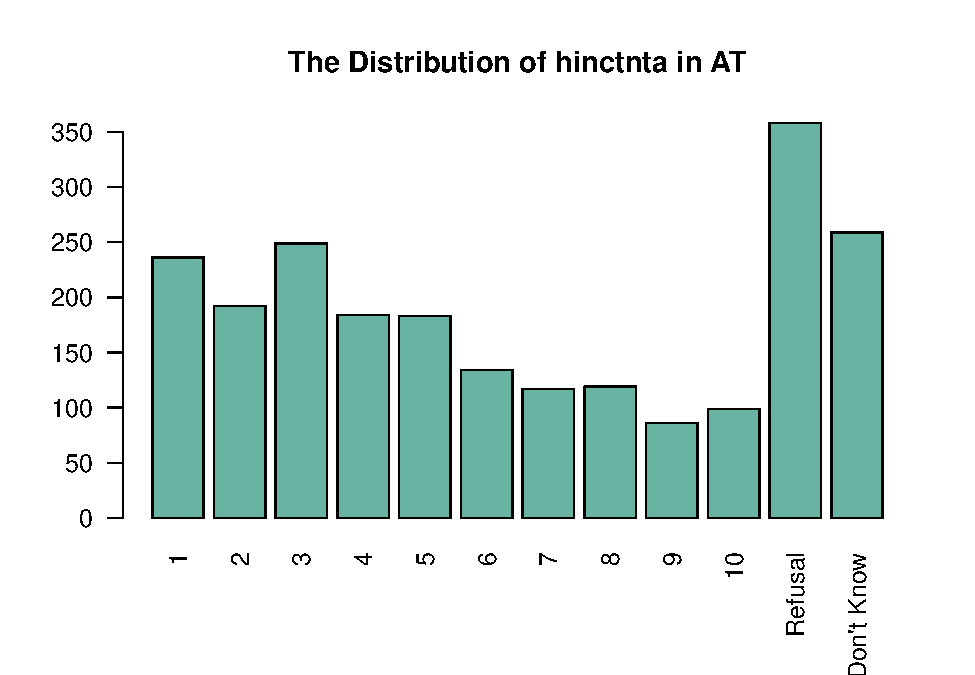
\includegraphics{finalreport_files/figure-latex/unnamed-chunk-12-1.pdf}

\begin{Shaded}
\begin{Highlighting}[]
\NormalTok{PT\_imp }\OtherTok{\textless{}{-}} \FunctionTok{mice}\NormalTok{(PT\_sub,}
               \AttributeTok{m =} \DecValTok{20}\NormalTok{,}
               \AttributeTok{maxit =} \DecValTok{10}\NormalTok{, }
               \AttributeTok{method =}\NormalTok{ meth,}
               \AttributeTok{predictorMatrix =}\NormalTok{ PT\_pred,}
               \AttributeTok{seed =} \DecValTok{12345}\NormalTok{,}
               \AttributeTok{print =} \ConstantTok{FALSE}\NormalTok{)}
\end{Highlighting}
\end{Shaded}

\begin{verbatim}
## Warning: Number of logged events: 2600
\end{verbatim}

\begin{Shaded}
\begin{Highlighting}[]
\CommentTok{\# Imputation for Poland}
\FunctionTok{vis\_miss}\NormalTok{(PL\_sub) }\CommentTok{\# Imputing m sets according to amount of percentage missing in income}
\end{Highlighting}
\end{Shaded}

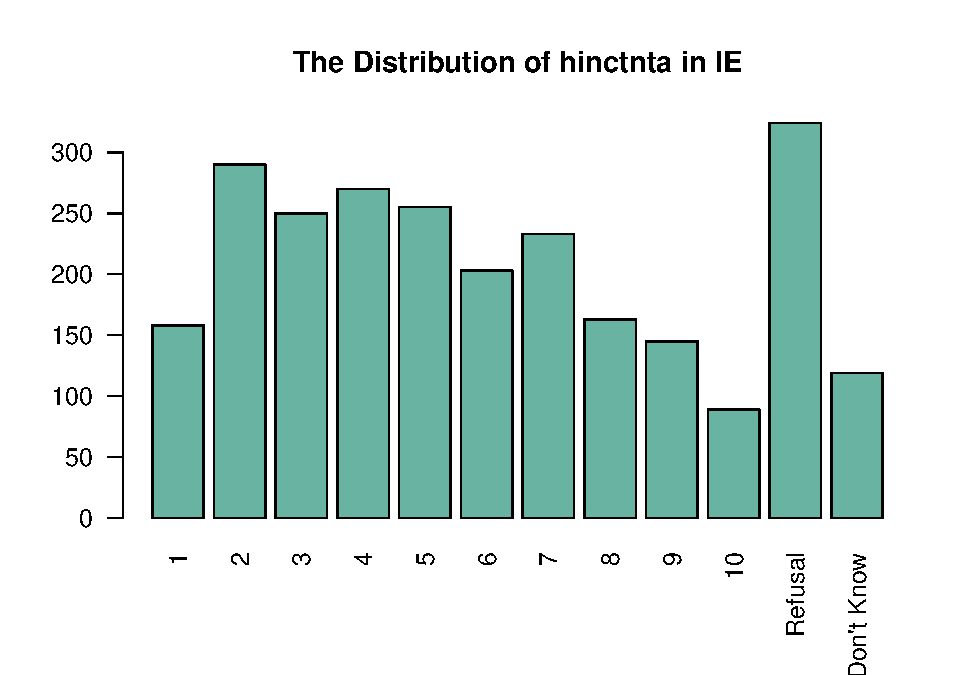
\includegraphics{finalreport_files/figure-latex/unnamed-chunk-12-2.pdf}

\begin{Shaded}
\begin{Highlighting}[]
\NormalTok{PL\_imp }\OtherTok{\textless{}{-}} \FunctionTok{mice}\NormalTok{(PL\_sub,}
               \AttributeTok{m =} \DecValTok{39}\NormalTok{,}
               \AttributeTok{maxit =} \DecValTok{10}\NormalTok{, }
               \AttributeTok{method =}\NormalTok{ meth,}
               \AttributeTok{predictorMatrix =}\NormalTok{ PL\_pred,}
               \AttributeTok{seed =} \DecValTok{12345}\NormalTok{,}
               \AttributeTok{print =} \ConstantTok{FALSE}\NormalTok{)}

\CommentTok{\# Imputation for Hungary}
\FunctionTok{vis\_miss}\NormalTok{(HU\_sub) }\CommentTok{\# Imputing m sets according to amount of percentage missing in income}
\end{Highlighting}
\end{Shaded}

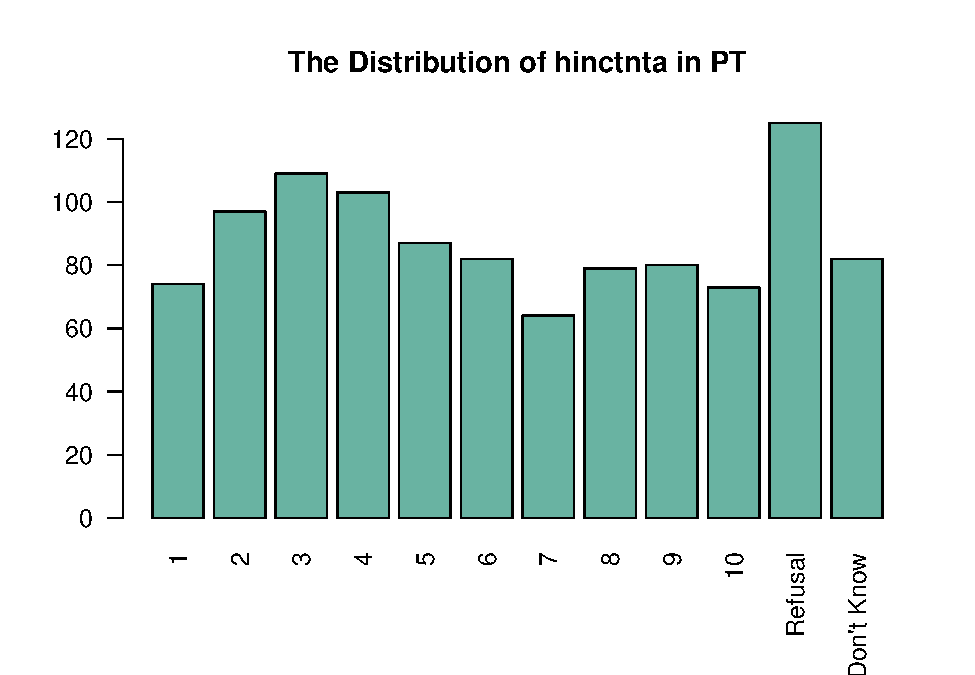
\includegraphics{finalreport_files/figure-latex/unnamed-chunk-12-3.pdf}

\begin{Shaded}
\begin{Highlighting}[]
\NormalTok{HU\_imp }\OtherTok{\textless{}{-}} \FunctionTok{mice}\NormalTok{(HU\_sub,}
               \AttributeTok{m =} \DecValTok{40}\NormalTok{,}
               \AttributeTok{maxit =} \DecValTok{10}\NormalTok{, }
               \AttributeTok{method =}\NormalTok{ meth,}
               \AttributeTok{predictorMatrix =}\NormalTok{ HU\_pred,}
               \AttributeTok{seed =} \DecValTok{12345}\NormalTok{,}
               \AttributeTok{print =} \ConstantTok{FALSE}\NormalTok{)}

\CommentTok{\# Imputation for Ireland}
\FunctionTok{vis\_miss}\NormalTok{(IE\_sub) }\CommentTok{\# Imputing m sets according to amount of percentage missing in income}
\end{Highlighting}
\end{Shaded}

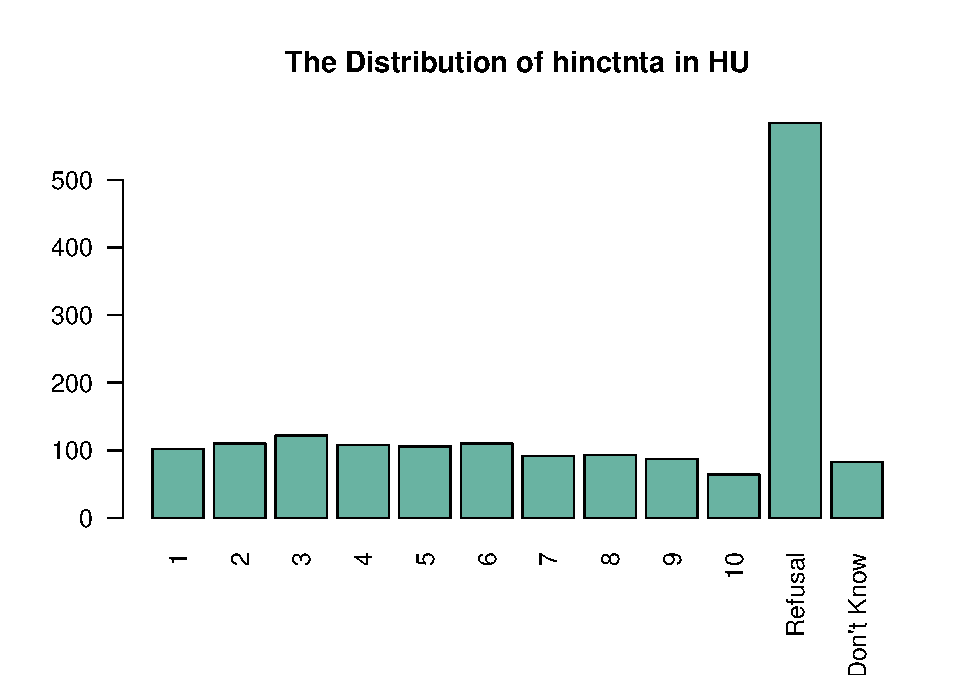
\includegraphics{finalreport_files/figure-latex/unnamed-chunk-12-4.pdf}

\begin{Shaded}
\begin{Highlighting}[]
\NormalTok{IE\_imp }\OtherTok{\textless{}{-}} \FunctionTok{mice}\NormalTok{(IE\_sub,}
               \AttributeTok{m =} \DecValTok{28}\NormalTok{,}
               \AttributeTok{maxit =} \DecValTok{10}\NormalTok{, }
               \AttributeTok{method =}\NormalTok{ meth,}
               \AttributeTok{predictorMatrix =}\NormalTok{ IE\_pred,}
               \AttributeTok{seed =} \DecValTok{12345}\NormalTok{,}
               \AttributeTok{print =} \ConstantTok{FALSE}\NormalTok{)}

\CommentTok{\# Imputation for Austria}
\FunctionTok{vis\_miss}\NormalTok{(AT\_sub) }\CommentTok{\# Imputing m sets according to amount of percentage missing in income}
\end{Highlighting}
\end{Shaded}

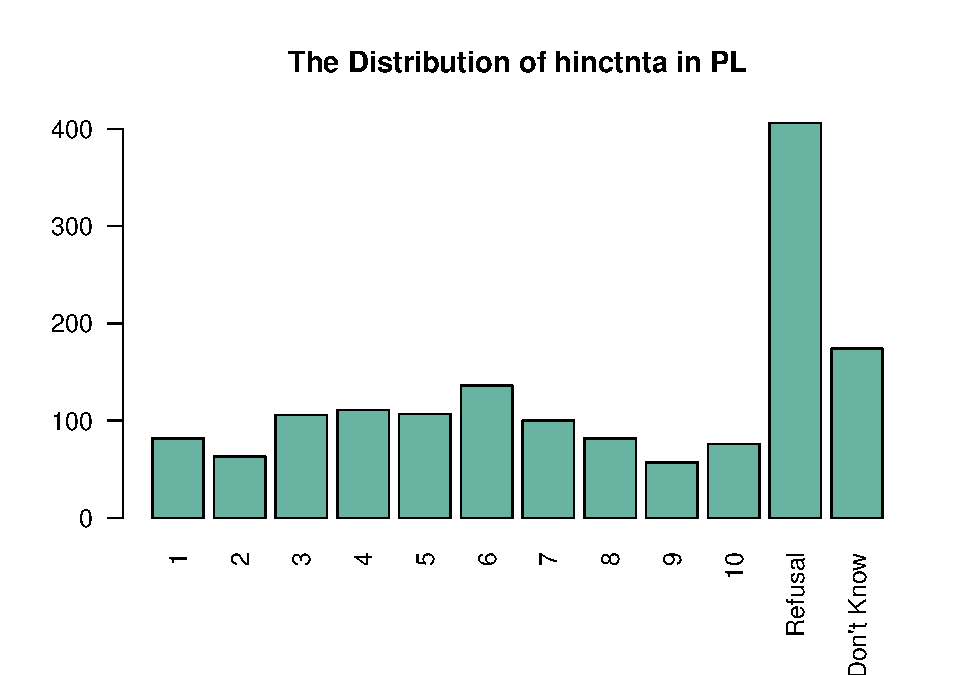
\includegraphics{finalreport_files/figure-latex/unnamed-chunk-12-5.pdf}

\begin{Shaded}
\begin{Highlighting}[]
\NormalTok{AT\_imp }\OtherTok{\textless{}{-}} \FunctionTok{mice}\NormalTok{(AT\_sub,}
               \AttributeTok{m =} \DecValTok{18}\NormalTok{,}
               \AttributeTok{maxit =} \DecValTok{10}\NormalTok{, }
               \AttributeTok{method =}\NormalTok{ meth,}
               \AttributeTok{predictorMatrix =}\NormalTok{ AT\_pred,}
               \AttributeTok{seed =} \DecValTok{12345}\NormalTok{,}
               \AttributeTok{print =} \ConstantTok{FALSE}\NormalTok{)}
\end{Highlighting}
\end{Shaded}

\hypertarget{checking-convergence}{%
\subsection{3.9 Checking convergence}\label{checking-convergence}}

\begin{Shaded}
\begin{Highlighting}[]
\CommentTok{\# Checking convergence for Portugal}
\FunctionTok{plot}\NormalTok{(PT\_imp)}
\end{Highlighting}
\end{Shaded}

\includegraphics{finalreport_files/figure-latex/unnamed-chunk-13-1.pdf}
\includegraphics{finalreport_files/figure-latex/unnamed-chunk-13-2.pdf}
\includegraphics{finalreport_files/figure-latex/unnamed-chunk-13-3.pdf}
\includegraphics{finalreport_files/figure-latex/unnamed-chunk-13-4.pdf}
\includegraphics{finalreport_files/figure-latex/unnamed-chunk-13-5.pdf}

\begin{Shaded}
\begin{Highlighting}[]
\FunctionTok{densityplot}\NormalTok{(PT\_imp)[}\DecValTok{4}\NormalTok{]}
\end{Highlighting}
\end{Shaded}

\begin{verbatim}
## Hint: Did you know, an equivalent figure can be created with `ggmice()`?
## For example, to plot a variable named 'my_vrb' from a mids object called 'my_mids', run: 
## 
##     ggmice(my_mids, ggplot2::aes(x = my_vrb, group = .imp)) +
##     ggplot2::geom_density() 
## 
## See amices.org/ggmice for more info.
\end{verbatim}

\includegraphics{finalreport_files/figure-latex/unnamed-chunk-13-6.pdf}

\begin{Shaded}
\begin{Highlighting}[]
\FunctionTok{bwplot}\NormalTok{(PT\_imp)[}\DecValTok{8}\NormalTok{]}
\end{Highlighting}
\end{Shaded}

\begin{verbatim}
## Hint: Did you know, an equivalent figure can be created with `ggmice()`?
## For example, to plot a variable named 'my_vrb' from a mids object called 'my_mids', run: 
## 
##     ggmice(my_mids, ggplot2::aes(x = .imp, y = my_vrb)) +
##     ggplot2::geom_boxplot() 
## 
## See amices.org/ggmice for more info.
\end{verbatim}

\includegraphics{finalreport_files/figure-latex/unnamed-chunk-13-7.pdf}

\begin{Shaded}
\begin{Highlighting}[]
\CommentTok{\# Outcome is midpoint of the median income class}
\NormalTok{PT\_imp }\SpecialCharTok{\%\textgreater{}\%} 
  \FunctionTok{complete}\NormalTok{(}\StringTok{\textquotesingle{}long\textquotesingle{}}\NormalTok{) }\SpecialCharTok{\%\textgreater{}\%} 
  \FunctionTok{with}\NormalTok{(}\FunctionTok{tapply}\NormalTok{(income, .imp, median)) }\SpecialCharTok{\%\textgreater{}\%} 
  \FunctionTok{median}\NormalTok{()}
\end{Highlighting}
\end{Shaded}

\begin{verbatim}
## [1] 13885
\end{verbatim}

\begin{Shaded}
\begin{Highlighting}[]
\CommentTok{\# Checking convergence for Poland}
\FunctionTok{plot}\NormalTok{(PL\_imp)}
\end{Highlighting}
\end{Shaded}

\includegraphics{finalreport_files/figure-latex/unnamed-chunk-13-8.pdf}
\includegraphics{finalreport_files/figure-latex/unnamed-chunk-13-9.pdf}
\includegraphics{finalreport_files/figure-latex/unnamed-chunk-13-10.pdf}
\includegraphics{finalreport_files/figure-latex/unnamed-chunk-13-11.pdf}
\includegraphics{finalreport_files/figure-latex/unnamed-chunk-13-12.pdf}

\begin{Shaded}
\begin{Highlighting}[]
\FunctionTok{densityplot}\NormalTok{(PL\_imp)[}\DecValTok{4}\NormalTok{]}
\end{Highlighting}
\end{Shaded}

\begin{verbatim}
## Hint: Did you know, an equivalent figure can be created with `ggmice()`?
## For example, to plot a variable named 'my_vrb' from a mids object called 'my_mids', run: 
## 
##     ggmice(my_mids, ggplot2::aes(x = my_vrb, group = .imp)) +
##     ggplot2::geom_density() 
## 
## See amices.org/ggmice for more info.
\end{verbatim}

\includegraphics{finalreport_files/figure-latex/unnamed-chunk-13-13.pdf}

\begin{Shaded}
\begin{Highlighting}[]
\FunctionTok{bwplot}\NormalTok{(PL\_imp)[}\DecValTok{8}\NormalTok{]}
\end{Highlighting}
\end{Shaded}

\begin{verbatim}
## Hint: Did you know, an equivalent figure can be created with `ggmice()`?
## For example, to plot a variable named 'my_vrb' from a mids object called 'my_mids', run: 
## 
##     ggmice(my_mids, ggplot2::aes(x = .imp, y = my_vrb)) +
##     ggplot2::geom_boxplot() 
## 
## See amices.org/ggmice for more info.
\end{verbatim}

\includegraphics{finalreport_files/figure-latex/unnamed-chunk-13-14.pdf}

\begin{Shaded}
\begin{Highlighting}[]
\CommentTok{\# Outcome is midpoint of the median income class}
\NormalTok{PL\_imp }\SpecialCharTok{\%\textgreater{}\%} 
  \FunctionTok{complete}\NormalTok{(}\StringTok{\textquotesingle{}long\textquotesingle{}}\NormalTok{) }\SpecialCharTok{\%\textgreater{}\%} 
  \FunctionTok{with}\NormalTok{(}\FunctionTok{tapply}\NormalTok{(income, .imp, median)) }\SpecialCharTok{\%\textgreater{}\%} 
  \FunctionTok{median}\NormalTok{()}
\end{Highlighting}
\end{Shaded}

\begin{verbatim}
## [1] 3950.5
\end{verbatim}

\begin{Shaded}
\begin{Highlighting}[]
\CommentTok{\# Checking convergence for Ireland}
\FunctionTok{plot}\NormalTok{(IE\_imp)}
\end{Highlighting}
\end{Shaded}

\includegraphics{finalreport_files/figure-latex/unnamed-chunk-13-15.pdf}
\includegraphics{finalreport_files/figure-latex/unnamed-chunk-13-16.pdf}
\includegraphics{finalreport_files/figure-latex/unnamed-chunk-13-17.pdf}
\includegraphics{finalreport_files/figure-latex/unnamed-chunk-13-18.pdf}
\includegraphics{finalreport_files/figure-latex/unnamed-chunk-13-19.pdf}
\includegraphics{finalreport_files/figure-latex/unnamed-chunk-13-20.pdf}

\begin{Shaded}
\begin{Highlighting}[]
\FunctionTok{densityplot}\NormalTok{(IE\_imp)[}\DecValTok{4}\NormalTok{]}
\end{Highlighting}
\end{Shaded}

\begin{verbatim}
## Hint: Did you know, an equivalent figure can be created with `ggmice()`?
## For example, to plot a variable named 'my_vrb' from a mids object called 'my_mids', run: 
## 
##     ggmice(my_mids, ggplot2::aes(x = my_vrb, group = .imp)) +
##     ggplot2::geom_density() 
## 
## See amices.org/ggmice for more info.
\end{verbatim}

\includegraphics{finalreport_files/figure-latex/unnamed-chunk-13-21.pdf}

\begin{Shaded}
\begin{Highlighting}[]
\FunctionTok{bwplot}\NormalTok{(IE\_imp)[}\DecValTok{8}\NormalTok{]}
\end{Highlighting}
\end{Shaded}

\begin{verbatim}
## Hint: Did you know, an equivalent figure can be created with `ggmice()`?
## For example, to plot a variable named 'my_vrb' from a mids object called 'my_mids', run: 
## 
##     ggmice(my_mids, ggplot2::aes(x = .imp, y = my_vrb)) +
##     ggplot2::geom_boxplot() 
## 
## See amices.org/ggmice for more info.
\end{verbatim}

\includegraphics{finalreport_files/figure-latex/unnamed-chunk-13-22.pdf}

\begin{Shaded}
\begin{Highlighting}[]
\CommentTok{\# Outcome is midpoint of the median income class}
\NormalTok{IE\_imp }\SpecialCharTok{\%\textgreater{}\%} 
  \FunctionTok{complete}\NormalTok{(}\StringTok{\textquotesingle{}long\textquotesingle{}}\NormalTok{) }\SpecialCharTok{\%\textgreater{}\%} 
  \FunctionTok{with}\NormalTok{(}\FunctionTok{tapply}\NormalTok{(income, .imp, median)) }\SpecialCharTok{\%\textgreater{}\%} 
  \FunctionTok{median}\NormalTok{()}
\end{Highlighting}
\end{Shaded}

\begin{verbatim}
## [1] 572.5
\end{verbatim}

\begin{Shaded}
\begin{Highlighting}[]
\CommentTok{\# Checking convergence for Hungary}
\FunctionTok{plot}\NormalTok{(HU\_imp)}
\end{Highlighting}
\end{Shaded}

\includegraphics{finalreport_files/figure-latex/unnamed-chunk-13-23.pdf}
\includegraphics{finalreport_files/figure-latex/unnamed-chunk-13-24.pdf}
\includegraphics{finalreport_files/figure-latex/unnamed-chunk-13-25.pdf}
\includegraphics{finalreport_files/figure-latex/unnamed-chunk-13-26.pdf}
\includegraphics{finalreport_files/figure-latex/unnamed-chunk-13-27.pdf}

\begin{Shaded}
\begin{Highlighting}[]
\FunctionTok{densityplot}\NormalTok{(HU\_imp)[}\DecValTok{4}\NormalTok{]}
\end{Highlighting}
\end{Shaded}

\begin{verbatim}
## Hint: Did you know, an equivalent figure can be created with `ggmice()`?
## For example, to plot a variable named 'my_vrb' from a mids object called 'my_mids', run: 
## 
##     ggmice(my_mids, ggplot2::aes(x = my_vrb, group = .imp)) +
##     ggplot2::geom_density() 
## 
## See amices.org/ggmice for more info.
\end{verbatim}

\includegraphics{finalreport_files/figure-latex/unnamed-chunk-13-28.pdf}

\begin{Shaded}
\begin{Highlighting}[]
\FunctionTok{bwplot}\NormalTok{(HU\_imp)[}\DecValTok{8}\NormalTok{]}
\end{Highlighting}
\end{Shaded}

\begin{verbatim}
## Hint: Did you know, an equivalent figure can be created with `ggmice()`?
## For example, to plot a variable named 'my_vrb' from a mids object called 'my_mids', run: 
## 
##     ggmice(my_mids, ggplot2::aes(x = .imp, y = my_vrb)) +
##     ggplot2::geom_boxplot() 
## 
## See amices.org/ggmice for more info.
\end{verbatim}

\includegraphics{finalreport_files/figure-latex/unnamed-chunk-13-29.pdf}

\begin{Shaded}
\begin{Highlighting}[]
\CommentTok{\# Outcome is midpoint of the median income class}
\NormalTok{HU\_imp }\SpecialCharTok{\%\textgreater{}\%} 
  \FunctionTok{complete}\NormalTok{(}\StringTok{\textquotesingle{}long\textquotesingle{}}\NormalTok{) }\SpecialCharTok{\%\textgreater{}\%} 
  \FunctionTok{with}\NormalTok{(}\FunctionTok{tapply}\NormalTok{(income, .imp, median)) }\SpecialCharTok{\%\textgreater{}\%} 
  \FunctionTok{median}\NormalTok{()}
\end{Highlighting}
\end{Shaded}

\begin{verbatim}
## [1] 214500
\end{verbatim}

\begin{Shaded}
\begin{Highlighting}[]
\CommentTok{\# Checking convergence for Austria}
\FunctionTok{plot}\NormalTok{(AT\_imp)}
\end{Highlighting}
\end{Shaded}

\includegraphics{finalreport_files/figure-latex/unnamed-chunk-13-30.pdf}
\includegraphics{finalreport_files/figure-latex/unnamed-chunk-13-31.pdf}
\includegraphics{finalreport_files/figure-latex/unnamed-chunk-13-32.pdf}
\includegraphics{finalreport_files/figure-latex/unnamed-chunk-13-33.pdf}
\includegraphics{finalreport_files/figure-latex/unnamed-chunk-13-34.pdf}
\includegraphics{finalreport_files/figure-latex/unnamed-chunk-13-35.pdf}

\begin{Shaded}
\begin{Highlighting}[]
\FunctionTok{densityplot}\NormalTok{(AT\_imp)[}\DecValTok{4}\NormalTok{]}
\end{Highlighting}
\end{Shaded}

\begin{verbatim}
## Hint: Did you know, an equivalent figure can be created with `ggmice()`?
## For example, to plot a variable named 'my_vrb' from a mids object called 'my_mids', run: 
## 
##     ggmice(my_mids, ggplot2::aes(x = my_vrb, group = .imp)) +
##     ggplot2::geom_density() 
## 
## See amices.org/ggmice for more info.
\end{verbatim}

\includegraphics{finalreport_files/figure-latex/unnamed-chunk-13-36.pdf}

\begin{Shaded}
\begin{Highlighting}[]
\FunctionTok{bwplot}\NormalTok{(AT\_imp)[}\DecValTok{8}\NormalTok{]}
\end{Highlighting}
\end{Shaded}

\begin{verbatim}
## Hint: Did you know, an equivalent figure can be created with `ggmice()`?
## For example, to plot a variable named 'my_vrb' from a mids object called 'my_mids', run: 
## 
##     ggmice(my_mids, ggplot2::aes(x = .imp, y = my_vrb)) +
##     ggplot2::geom_boxplot() 
## 
## See amices.org/ggmice for more info.
\end{verbatim}

\includegraphics{finalreport_files/figure-latex/unnamed-chunk-13-37.pdf}

\begin{Shaded}
\begin{Highlighting}[]
\CommentTok{\# Outcome is midpoint of the median income class}
\NormalTok{AT\_imp }\SpecialCharTok{\%\textgreater{}\%} 
  \FunctionTok{complete}\NormalTok{(}\StringTok{\textquotesingle{}long\textquotesingle{}}\NormalTok{) }\SpecialCharTok{\%\textgreater{}\%} 
  \FunctionTok{with}\NormalTok{(}\FunctionTok{tapply}\NormalTok{(income, .imp, median)) }\SpecialCharTok{\%\textgreater{}\%} 
  \FunctionTok{median}\NormalTok{()}
\end{Highlighting}
\end{Shaded}

\begin{verbatim}
## [1] 34050
\end{verbatim}

\hypertarget{iv.-conclusion}{%
\section{IV. Conclusion}\label{iv.-conclusion}}

\end{document}
